\documentclass[11pt,times,letter]{article}


\topmargin=-0.5in    % Make letterhead start about 1 inch from top of page
\textheight=8.5in  % text height can be bigger for a longer letter
\oddsidemargin=0pt % leftmargin is 1 inch
\textwidth=6.4in   % textwidth of 6.5in leaves 1 inch for right margin

\usepackage{amsmath, amsfonts,amsthm,amssymb,bm}
\usepackage{dsfont}

\usepackage[english]{babel}

\newcommand{\cyan}[1]{{ \color{cyan} {{#1} }}}
\usepackage[normalem]{ulem}
\newcommand{\xcyan}[1]{{\color{cyan}{{\sout{{#1} }}}}}
\newcommand{\xxcyan}[1]{{\color{cyan}{{\xout{{#1} }}}}}

\usepackage{latexsym,amssymb,amsfonts,graphicx}
\usepackage{amsmath,dsfont}
\usepackage{verbatim}
\usepackage{mathrsfs}
\usepackage{bm}
\usepackage{color}
\usepackage{epsfig}
\usepackage{subfigure}

\setlength{\parskip}{1ex plus 0.5ex minus 0.2ex}
\usepackage{url}
\usepackage{bm}
\usepackage{natbib}

\usepackage[colorlinks,linkcolor=blue,citecolor=blue,anchorcolor=blue]{hyperref}

\usepackage{tikz}
\usetikzlibrary{arrows.meta, positioning}

\newcommand{\idc}{\mathbf{1}}
\newcommand{\Px}{ \mathbb{P} }
\newcommand{\Qx}{ \mathbb{Q} }
\newcommand{\N}{ \mathbb{N} }
\newcommand{\Ex}{ \mathbb{E} }
\newcommand{\gt}{\mathcal{G}_t}
\newcommand{\Zx}{\mathbb{Z}}

\def\esssup_#1{\underset{#1}{\mathrm{ess\,sup\, }}}
\def\essinf_#1{\underset{#1}{\mathrm{ess\,inf\, }}}
\def\argmax_#1{\underset{#1}{\mathrm{arg\,max\, }}}
\def\argmin_#1{\underset{#1}{\mathrm{arg\,min\, }}}

\newcommand{\A}{{\cal A}}
\newcommand{\cA}{\mathcal{A}}
\newcommand{\DP}{\mbox{DP}}
\newcommand{\PIRS}{\mbox{Pirs}}

\newcommand{\Hx}{\mathbb{H}}
\newcommand{\Gx}{\mathbb{G}}
\newcommand{\Fx}{\mathbb{F} }
\newcommand{\cO}{\mathcal{O}}
\newcommand{\cL}{\mathcal{L}}
\newcommand{\D}{\mathrm{d}}
\newcommand{\too}{-\!\!\!\to}

\newcommand{\F}{\mathcal{F}}
\newcommand{\G}{\mathcal{G}}
\newcommand{\R}{\mathds{R}}
\newcommand{\taue}{\tau_{\varepsilon}^t}
\newcommand{\T}{\top}
\newcommand{\AZ}{{\bf(A$_{Z}$)}}
\newcommand{\Af}{{\bf(A$_{f}$)}}
\newcommand{\Afb}{{\bf(A$_{fb}$)}}
\newcommand{\Asc}{{\bf(A$_{s3}$)}}
\newcommand{\Aga}{{\bf(A$_{ga}$)}}
\newcommand{\C}{{\tt{C}}}

\newtheorem{theorem}{Theorem}[section]
\newtheorem{definition}{Definition}[section]
\numberwithin{equation}{section}

\newtheorem{proposition}[theorem]{Proposition}
\newtheorem{remark}[theorem]{Remark}
\newtheorem{lemma}[theorem]{Lemma}
\newtheorem{corollary}[theorem]{Corollary}
\newtheorem{example}{Example}[section]
\allowdisplaybreaks[4]

\definecolor{Red}{rgb}{1.00, 0.00, 0.00}
\newcommand{\Red}{\color{Red}}
\definecolor{DRed}{rgb}{0.5, 0.00, 0.00}
\newcommand{\DRed}{\color{DRed}}
\definecolor{Blue}{rgb}{0.00, 0.00, 1.00}
\newcommand{\Blue}{\color{Blue}}
\definecolor{Green}{rgb}{0.0, 0.4, 0.0}
\newcommand{\Green}{\color{Green}}
\newcommand{\Yellow}{\color{yellow}}


\title{ Mean Field Game of Optimal Tracking Portfolio}
\author{Lijun Bo \thanks{Email: lijunbo@ustc.edu.cn, School of Mathematics and Statistics, Xidian University, Xi'an, 710126, China.}
\and
Yijie Huang \thanks{Email: huang1@mail.ustc.edu.cn, School of Mathematical Sciences, University of Science and Technology of China, Hefei, 230026, China.}
\and
Xiang Yu \thanks{Email: xiang.yu@polyu.edu.hk, Department of Applied Mathematics, The Hong Kong Polytechnic University, Kowloon, Hong Kong, China.}
}

\date{\vspace{-0.5in}}
\begin{document}
\maketitle

\begin{abstract}
This paper studies the mean field game (MFG) problem arising from a large population competition in fund management, featuring a new type of relative performance via the benchmark tracking constraint. In the $n$-agent model, each agent can strategically inject capital to ensure that the total wealth outperforms the benchmark process, which is modeled as a linear combination of the population's average wealth process and an exogenous  market index process. That is, each agent is concerned about the performance of her competitors captured by the floor constraint. With a continuum of agents, we formulate the constrained MFG problem and transform it into an equivalent unconstrained MFG problem with a reflected state process. We establish the existence of the mean field equilibrium (MFE) using the PDE approach. Firstly, by applying the dual transform, the best response control of the representative agent can be characterized in analytical form in terms of a dual reflected diffusion process. As a novel contribution, we verify the consistency condition of the MFE in separated domains with the help of the duality relationship and properties of the dual process.\\
\ \\
\textbf{Keywords}: Mean field game, relative tracking portfolio, mean field equilibrium, dual reflected diffusion process, fixed point     
\end{abstract}

\vspace{0.1in}
\section{Introduction}
Portfolio  management with benchmark tracking has been an active research topic in quantitative finance, which involves constructing a portfolio that closely tracks a chosen benchmark.  The goal is usually to minimize the tracking error (for instance, the variance or downside variance relative to the index value or return). Some related studies along this direction can be found in \cite{Browne9,Browne99,Browne00}, \cite{Gaivoronski05},  \cite{YaoZZ06}, \cite{Strub18}, \cite{NLFC}, among others.  Recently,  \cite{BoLiaoYu21} proposes a tracking formulation using the (fictitious) capital injection to outperform the benchmark process. The fictitious injected capital can also be regarded as a risk measure of the expected largest shortfall with reference to the benchmark. Later, this relaxed benchmark tracking formulation has been further generalized to the Merton consumption problem under different types of benchmark processes in \cite{BHY23,BHY24a,BHY24b} and to the incomplete market model using the continuous-time.

In the present paper, we study the relaxed tracking portfolio using capital injection in the mean field game (MFG) framework. In particular, we consider n competitive agents who concern their relative performance with respect to the population's average wealth process.  When the number of agents n goes to infinity, we study the corresponding MFG problem that is more tractable. Introduced independently by  \cite{Huang06} and \cite{Lasry07}, MFGs have emerged as a significant research area in recent years, serving as a powerful tool for studying  large population games. The existing literature on n-player and mean filed portfolio games on relative performance mostly consider the utilities defined on the comparison between the agent's own wealth and the population's average wealth. To name a few,  \cite{Espinosa15} consider the $n$-agents and MFG game problem and obtain the existence and uniqueness of a Nash equilibrium under general utility and portfolio constraints; Lacker and  \cite{Lacker19} study both n-player and mean field games of optimal portfolio management under competition and constant relative risk aversion (CRRA) or constant absolute risk aversion (CARA) relative performance criteria, which can be explicitly solved;  \cite{Lacker20} generalize the optimal investment problem under CRRA utility to include consumption;  \cite{FuZhou23} extend the results in \cite{Lacker19} by allowing random return rate and volatility, and solve the MFG  by the martingale optimality principle approach, such that the unique Nash equilibrium can be  characterized in terms of a mean field FBSDE; By applying master equation approach,  \cite{Souganidis24}  consider a MFG of optimal investment  with relative performance concerns, derive the MFG solution and use the mean field solution to approximate their counterparts in the n-player game;  \cite{BWY24a} examine the equilibrium consumption under linear and multiplicative external habit formation in the framework of mean field relative performance;  \cite{BWY24b} recently consider the mean field game under the CRRA relative performance on terminal wealth in the model with contagious jump risk.

In contrast, we consider a new type of relative performance in the sense that each agent incorporates the population's average wealth into the benchmark constraint. That is, each agent needs to strategically choose the investment strategy and capital injection to ensure that her own wealth process always dominates the benchmark process involving the population's average wealth. The goal of each agent is to minimize the expectation of the accumulated capital injection. After some equivalent transformations, we need to solve a type of MFG with state reflection at zero. Note that although mean field games have received significant attention, the research on MFG with reflected state process is underexplored. \cite{Bayraktar2019} formulate a MFG problem with drift-controlled diffusion process with reflections for large symmetric queuing systems in heavy traffic with strategic servers. By using master equation approach,  \cite{Ricciardi2023} study the convergence of Nash equilibrium in an n-player differential game towards the optimal strategies in the MFGs for drift control problem with reflection. Recently,  \cite{BWY25} explore a MFG problem with state-control joint law dependence and the reflected state process, in which the existence of MFEs is established by developing the compactification method and the connections between the MFG and the n-player game problems are also discussed.  

In this work, we solve the MFG with state reflections by using the analytical approach. In the first step, we fix a deterministic differentiable function that represents the average wealth, and study the optimization problem of the representative agent. By introducing  an auxiliary controlled state process with reflection, we reformulate the control problem with fictitious singular control of capital injection under floor constraint as a unconstrained regular control problem. By means of the dual transform, probabilistic representation and stochastic flow analysis, the existence of classical solution to the HJB equation is obtained and the verification theorem on the best response control is presented. Then, we aim to  verify the consistency condition and find an MFE in the second step based on the characterization of the value function and feedback function of the best response control derived in the pervious step. It is sufficient to show the existence of the fixed point for the mapping that stems from the consistency condition. The difficulty lies in the complicated expression of the mapping on the controlled state variable and the special piecewise form that depends on input of the mapping. In response, we introduce the reflected dual process, which help to provide a probability representation of best response portfolio strategy and establish the existence and uniqueness of the fixed point of the dual variable. Then, we return to the primal state variable by using the dual relationship and find the MFE in piecewise form by constructing the fixed point. We split the domain into two regions depending on the model parameters, the initial level of the wealth and benchmark processes and the time horizon: on the non-capital injection region, we derive the explicit expression of the optimal investment strategy and extra capital injection is unnecessary; on the capital injection region, not explicit but calculable representations of the optimal investment and capital injection strategies are provided. The road map of our proposed approach based on the auxiliary process and the dual process is summarized in the flow chart.  

{\footnotesize
\begin{center}
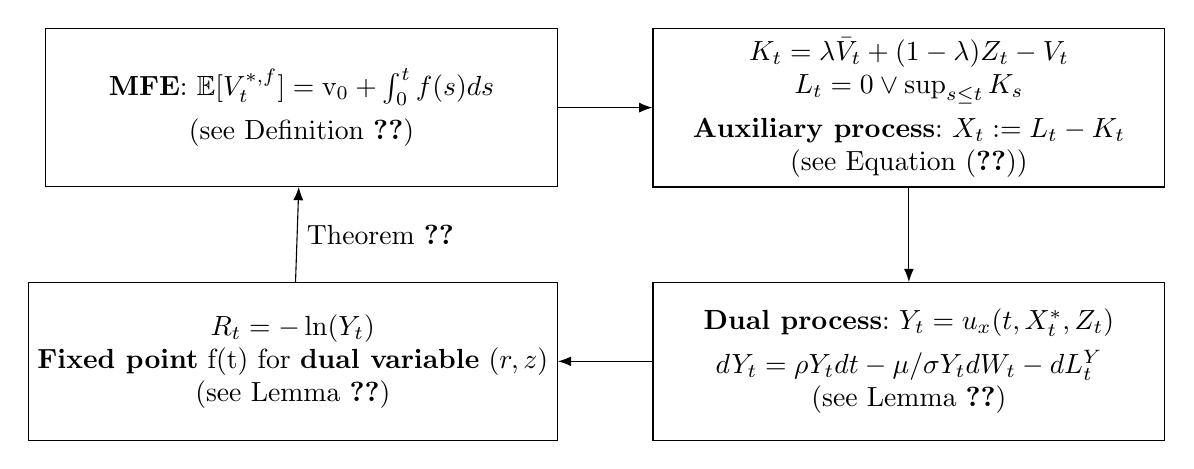
\begin{tikzpicture}[
    node distance=1.2cm,
    box/.style={draw, rectangle, minimum width=6.5cm, minimum height=2cm, align=center}
]
    \node[box] (def) {{\bf MFE}:~$\Ex[V_t^{*,f}]=\mathrm{v}_0+\int_0^t f(s)ds$\\[0.4em] (see  Definition \ref{def:MFG})};
    \node[box, right=of def] (xt) {$K_t=\lambda \bar{V}_t+(1-\lambda )Z_t-V_t$\\ $L_t=0\vee \sup_{s\leq t}K_s$\\[0.4em] {\bf Auxiliary process}:~$X_t:=L_t-K_t$ \\(see Equation \eqref{state-X})};
    \node[box, below=of xt] (ft) {{\bf Dual process}:~$Y_t=u_x(t,X_t^*,Z_t)$\\[0.4em] $dY_t= \rho Y_tdt-\mu/\sigma Y_tdW_t-dL_t^Y$\\(see Lemma \ref{lem:dual-process})};
    \node[box, left=of ft] (int) {$R_t=-\ln(Y_t)$\\ {\bf Fixed point} f(t) for {\bf dual variable} $(r,z)$\\ (see Lemma \ref{lem:fixpoint-r})};


    \draw[-Latex] (def) -- (xt);
    \draw[-Latex] (xt) -- (ft);
    \draw[-Latex] (ft) -- (int);
    \draw[-Latex] (int) -- (def)
     node[midway, right] { Theorem \ref{thm:MF-equilibrium}};
\end{tikzpicture}
\end{center}}

The remainder of the paper is organized as follows. Section \ref{sec:model} introduces the finite-agent and MFG problems of the optimal tracking portfolio. Section \ref{sec:auxiliary} proposes an auxiliary state process with reflection and derive the associated HJB equation with Neumann boundary condition for the best response control problem, in which the best response portfolio process of the representative agent can be obtained in analytical form in terms of a dual reflected diffusion process. Section \ref{sec:MFG}  verifies the consistency condition and establishes the existence of the MFE with the aid of an auxiliary reflected dual process. Section \ref{sec:numerical} presents some quantitative properties and numerical examples of the MFE. The proofs of the main results in previous sections are collected in Section \ref{sec:proofs}.

\section{Finite-Agent and Mean Field Game Problems}\label{sec:model}

Let $(\Omega,\F,\Fx,\Px)$ be a filtered probability space with the filtration $\Fx=(\F_t)_{t\in[0,T]}$ satisfying the usual conditions. We consider a financial market consisting of $n$ agents, in which the $i$-th agent invest her wealth in the $i$-th risky asset whose price dynamics is given by 
\begin{equation}\label{eq:stock}
  \frac{d S_t^i}{S_{t}^i} = \mu dt +\sigma dW_t^i,\quad t\in [0,T],
\end{equation}
where the return rate $\mu>0$ and the volatility  $\sigma>0$. Here, $(W^1,\ldots,W^n)=(W_t^1,\ldots,W_t^n)^{\top}_{t\in[0,T]}$ is an $n$-dimensional Brownian motion, specified to each individual risky asset, standing for the idiosyncratic noise. It is assumed that the riskless interest rate $r=0$, which amounts to the change of num\'{e}raire. From this point onwards, all processes including the wealth process and the benchmark process are defined after the change of num\'{e}raire. At time $t\geq0$, let $\theta_t^i$ be the amount of wealth that the agent $i$ allocates in the stock $S^i$. The self-financing wealth process of agent $i$ satisfies the following controlled SDE:
 \begin{align}\label{eq:Vt}
dV_t^i=\theta^i_t \mu dt+\theta^i_t\sigma dW_t^i,\quad t\in [0,T].
\end{align}

We consider the relaxed benchmark tracking using the capital injection for each agent in the market.  At any time $t\geq0$, it is
 assumed that agent $i$ can strategically inject capital at such that the total wealth $V_t^i+C_t^i$
satisfies the relaxed constraint w.r.t. the linear combination of the average wealth process $\overline{V}_t^n=\frac{1}{n}\sum_{i=1}^n V^i_t$  and the market index process $Z_t^i$ that agent $i$ is concerned. The interaction of $n$ agents occurs through the average wealth process $\overline{V}^n_t$ in the relaxed constraint, which depicts the relative performance concern by the agent $i$ with respect to other peers. That is, after the injection of capital $C^i=(C_t^i)_{t\in[0,T]}$, each agent requires the total fund account $V_t^i+C_t^i$ to stay above the benchmark process $\lambda \overline{V}_t^n+(1-\lambda)Z_t^i$ for $\lambda \in(0,1)$ at all times $t\in[0,T]$. The market index process  $Z^i=(Z_t^i)_{t \in [0,T]}$, for $i=1,...,n$, is described as the following geometric Brownian motion (GBM) that
\begin{align}\label{eq:Zt-n}
d Z_t^i=\mu_Z Z_t^i d t+\sigma_Z Z_t^i d W_t^{i}, \quad Z_0^i=z\geq0,
\end{align}
where the return rate $\mu_Z>0$ and the volatility $\sigma_Z>0$ which satisfies $\frac{\mu_Z}{\sigma_Z}>\frac{\mu}{\sigma}$. Mathematically speaking, agent $i$ now aims to minimize the cumulative capital injected at the terminal time $T$, for $i=1,\ldots,n$, 
\begin{align}\label{eq:n-player}
\begin{cases}
\displaystyle {\rm w}^i(\mathrm{v},z):=\text{$\inf_{(\theta, C)\in\mathbb{U}} \Ex\left[ C_0^i+\int_0^{T} e^{-\rho t}dC^i_t\Big|V^i_0=\mathrm{v},Z_0^i=z\right]$}\\[1em]
\displaystyle \text{subjecting to\ \  $\lambda \overline{V}_t^n+(1-\lambda)Z_t^i\le V^i_t+C^i_t$ for all $t\in [0,T]$,}
\end{cases}
\end{align}
where $\lambda \in(0,1)$  represents the competition weight of agent $i$ towards her relative performance concern. The admissible control set $\mathbb{U}$ is defined as:
\begin{align*}
&\mathbb{U}:=\big\{\text{$(\theta,C)=(\theta_t,C_t)_{t\in[0,T]}$;~ $\theta$ is $\Fx$-adapted processes taking values on $\R$, $C$ is a non-negative,}\\
&\qquad\quad\text{ non-decreasing process with r.c.l.l. paths}\big\}.
\end{align*}
Here, for technical convenience, we assume that the initial wealth of each agent and the initial level of market index process are the same constants $(\mathrm{v},z)\in \R_+\times (0,\infty)$. 
 
With continuum of agents, we can consider the mean field game (MFG) problem as $n\rightarrow\infty$. Let us denote $\overline{V}=(\overline{V}_t)_{t\in[0,T]}$ by the average wealth of the mean field population. When $n\rightarrow\infty$, we expect that $[0,T]\ni t\mapsto\overline{V}_t$ is a deterministic differentiable function with the form $d\overline{V}_t=f(t)dt$ for some positive $f\in\C([0,T])$ and $\overline{V}_0=\mathrm{v}>0$. Here, $\C([0,T])$ denotes the set of real-valued continuous functions on $[0,T]$. Then, our MFG problem is to find $(\theta^*,C^*)=(\theta_t^*,C_t^*)_{t\in[0,T]}$ such that the best response satisfies the so-called consistency condition. 


For a given function $t\mapsto f(t)$ (or $t\mapsto\overline{V}_t$), we first consider the stochastic control problem for a representative agent that  
\begin{align}\label{eq:mfg}
\begin{cases}
\displaystyle {\rm w}(\mathrm{v},z):=\text{$\inf_{(\theta,C)\in \mathbb{U}} \Ex\left[ C_0+ \int_0^{T} e^{-\rho t}dC_t\Big|V_0^{\theta}=\mathrm{v},Z_0=z \right]$}\\[1em]
\displaystyle \text{subjecting to\ \  $\lambda \overline{V}_t +(1-\lambda )Z_t\le V_t^{\theta}+C_t$ for all $t\in [0,T]$,}
\end{cases}
\end{align}
where the wealth process $V$ of the representative agent satisfies that
\begin{align}\label{eq:Vt-MFG}
dV_t^{\theta}=\theta_t \mu dt+\theta_t\sigma dW_t,\quad t\in (0,T],\quad V_0^{\theta}=\mathrm{v}>0,
\end{align}
and the market index process $Z=(Z_t)_{t \in [0,T]}$ of the representative agent is given by
\begin{align}\label{eq:Zt-MFG}
d Z_t=\mu_Z Z_t d t+\sigma_Z Z_t d W_t,\quad Z_0=z\geq0.
\end{align}

We next give the definition of the mean field equilibrium for our MFG problem:
\begin{definition}[Mean Field Equilibrium]\label{def:MFG}
For a given function $f\in\C([0,T])$, let $(\theta^{*,f},C^{*,f})=(\theta_t^{*,f},C_t^{*,f})_{t\in[0,T]}\in \mathbb{U}$ be the best response solution to the stochastic control problem \eqref{eq:mfg} for the representative agent. The strategy $(\theta^{*,f},C^{*,f})$ is called a mean field equilibrium (MFE) if it is the best response to itself such that $\Ex[V_t^{*,f}]=\mathrm{v}_0+\int_0^t f(s)ds$ for all $t\in[0,T]$, where $V^{*,f}=(V_t^{*,f})_{t\in[0,T]}$ is the wealth process \eqref{eq:Vt-MFG} under the portfolio strategy $\theta^{*,f}$. 
\end{definition}
Based on the above definition, finding an MFE is to solve the following two-step problem:
\begin{itemize} 
\item {\bf Step 1.}~ For a given deterministic positive function $f\in\C([0,T])$, we solve the stochastic control problem \eqref{eq:mfg} for a representative agent against the fixed environment.
The best response strategy for the representative agent is denoted by $(\theta^{*,f},C^{*,f})\in \mathbb{U}$ and $V^{*,f}=(V_t^{*,f})_{t\in[0,T]}$ stands for the wealth process in \eqref{eq:Vt-MFG} under the strategy $\theta^{*,f}=(\theta_t^{*,f})_{t\in[0,T]}$.
\item{\bf Step 2.}~ We derive an MFE by using the consistency condition, which is equivalent to finding a fixed point $f^*\in\C([0,T])$ taking values on $\R_+$ to the fixed point problem $\Ex[V_t^{*,f}]=\mathrm{v}_0+\int_0^t f(s)ds$ for all $t\in[0,T]$. Then, the expected MFE is given by $(\theta^{*,f^*},C^{*,f^*})=(\theta_t^{*,f^*},C_t^{*,f^*})_{t\in[0,T]}$.
\end{itemize}



\section{Equivalent Problem Formulation for Best Response Control}\label{sec:auxiliary}

To tackle the best response control of the representative agent in problem \eqref{eq:mfg} with the floor constraint, we first reformulate the problem based on the observation that, for a fixed control $\theta$, the optimal $C$ is always the smallest adapted right-continuous and non-decreasing process that dominates $\lambda \overline{V}_t +(1-\lambda )Z_t-V_t^{\theta}$. It follows from Lemma 2.4 in \cite{BoLiaoYu21} that,  for a fixed regular control $\theta=(\theta_t)_{t\in[0,T]}$, the optimal singular control satisfies $C^{\theta,*}_t =0\vee \sup_{s\leq t}\left(\lambda \overline{V}_s +(1-\lambda )Z_s-V_{s}^{\theta}\right)$, $\forall t\in [0,T]$. Thus, the control problem \eqref{eq:mfg} admits the equivalent formulation as an unconstrained control problem with a running maximum cost that
\begin{align}\label{eq_orig_pb-mfg}
\hat{{\rm w}}(\mathrm{v},z)&=(1-\lambda)(z-\mathrm{v})^+\nonumber\\
&\quad+\inf_{\theta\in\mathbb{U}^{\rm r}}\ \Ex\left[ \int_0^{T} e^{-\rho t} d\left(0\vee \sup_{s\leq t}\left(\lambda \overline{V}_s +(1-\lambda )Z_s-V_{s}^{\theta}\right)\right)\right],
\end{align}
where $\mathbb{U}^{\rm r}$ denotes the admissible control set of the regular strategies $\theta=(\theta_t)_{t\in[0,T]}$ that will be specified later.

To formulate the auxiliary stochastic control problem, we will introduce a new controlled state
process to replace the process. Let $K_t:=\lambda \bar{V}_t+(1-\lambda )Z_t-V_t$ and define $L_t=0\vee \sup_{s\leq t}K_s$ for $t\in[0,T]$. Then, we define a new state process with reflection that $X_t:=L_t-K_t$ and 
\begin{align}\label{state-X}
dX_t=(\theta_t \mu -\lambda f(t)-(1-\lambda)\mu_Z Z_t)dt+(\theta_t\sigma-(1-\lambda)\sigma_Z Z_t )dW_t+dL_t,\quad t\in (0,T]
\end{align}
with $X_0=x=((1-\lambda)(\mathrm{v}-z))_+\in\R_+$. In particular, the process $L=(L_t)_{t\in[0,T]}$ which is referred to as the local time of $X$, it increases at time $t$ if and only if $X_t=0$, i.e., $L_t=D_t$. We will change the notation from $L_t$ to $L_t^X$ from this point on wards to emphasize its dependence on the new state process $X$ given in \eqref{state-X}.

We then need to solve an equivalent stochastic control problem, for $(t,x,z)\in[0,T]\times\R_+^2$, 
\begin{align}\label{eq_mfg-2}
&u(t,x,z):=\text{$\sup_{\theta\in \mathbb{U}_t^r} \Ex\left[  -\int_t^{T} e^{-\rho (s-t)}dL_s^X\Big|X_t=x,Z_t=z \right]$},
\end{align}
where the admissible control set $\mathbb{U}_t^{\rm r}$ is specified as the set of $\Fx$-adapted control processes $\theta=(\theta_s)_{s\in[t,T]}$ such that the reflected SDE \eqref{state-X} has a unique strong solution. The admissible control set $\mathbb{U}^{\rm r}$ given in \eqref{eq_orig_pb-mfg} satisfies $\mathbb{U}^{\rm r}=\mathbb{U}^{\rm r}_0$. 
It is straightforward to derive the next result:
\begin{lemma}\label{lem:propoertyu}
Let $(t,z)\in[0,T]\times \R_+$ be fixed. Then, the value function $x\mapsto u(t,x,z)$ given by \eqref{eq_mfg-2} is non-decreasing. Moreover, for all $(t,x_1,x_2,z)\in[0,T]\times \R_+^3$, we have
\begin{align}\label{eq:lipvx}
\left|u(t,x_1,z)-u(t,x_2,z)\right|\leq  |x_1-x_2|.
\end{align}
\end{lemma}


Denote by $\mathcal{D}_T:=[0,T)\times \R_+^2$ and $\overline{\mathcal{D}}_T:=[0,T]\times \R_+^2$. In what follows, let us first assume that the value function $u$ satisfies ${\C}^{1,2}(\mathcal{D}_T)\cap {\C}\left(\overline{\mathcal{D}}_T\right)$ and $u_{xx} < 0 $ on $\mathcal{D}_T$, which will be discussed and verified later. By heuristic dynamic programming argument, the HJB equation can be derived by
\begin{align}\label{HJB}
\begin{cases}
\displaystyle u_t+\sup_{\theta\in\R}\left[u_x\mu\theta+\frac{1}{2}u_{xx}(\sigma\theta-(1-\lambda)\sigma_Zz)^2+u_{xz}(\sigma\theta-(1-\lambda)\sigma_Zz)\sigma_Z z \right] \\[0.6em]
\displaystyle \qquad\qquad-((1-\lambda)\mu_Zz+\lambda f(t)) u_x+\mu_Z zu_z+\frac{1}{2}\sigma_Z^2z^2u_{zz}=\rho u,\quad \forall(t,x,z)\in\mathcal{D}_T,\\[0.6em]
\displaystyle u_x(t,0,z)=1,\quad \forall(t,z)\in[0,T)\times \R_+,\\[0.6em]
\displaystyle u(T,x,z)=0,\quad \forall(x,z)\in\R_+^2.
\end{cases}
\end{align}
The Neumann boundary condition $u_x(t,0,z)=1$ stems from the fact that $L_t^X$ increases if and only if $X_t=0$. 
 By taking the first order condition over the control,  we get
\begin{align}\label{HJB-nonlinear}
 &u_t-\frac{\mu^2}{2\sigma^2}\frac{u_x^2}{u_{xx}}-\frac{\mu\sigma_Z z}{\sigma}\frac{u_xu_{xz}}{u_{xx}}+\frac{1}{2}\sigma_Z^2z^2\left(u_{zz}-\frac{u_{xz}^2}{u_{xx}}\right)+\mu_Z zu_z\\
 &\qquad\qquad\qquad\quad-\left(\frac{(1-\lambda)(\mu_Z\sigma-\mu\sigma_Z)}{\sigma}z+\lambda f(t)\right)u_x =\rho u,\quad \forall(t,x,z)\in\mathcal{D}_T.\nonumber
\end{align}
Note that PDE \eqref{HJB-nonlinear} is fully nonlinear.  We first apply the dual transform to linearize the original HJB equation \eqref{HJB-nonlinear}. As a direct result of Lemma~\ref{lem:propoertyu},  $|u_x(t,x,z)|= u_x(t,x,z)\leq 1$ for all $(t,x,z)\in\overline{\mathcal{D}}_T$. Then, we may apply Legendre-Fenchel transform of the solution $u$ only w.r.t. $x$ that, for all $(t,y,z)\in[0,T]\times (0,1]\times\R_+$,
\begin{align}\label{eq:LFT-u}
\hat{u}(t,y,z):=\sup_{x>0}\{u(t,x,z)-xy\}. 
\end{align}
Consequently $u(t,x,z)=\inf_{y\in(0,1]}\{\hat{u}(t,y,z)+xy\}$ for $(t,x,z)\in\overline{\mathcal{D}}_T$. Define that $x^*(t,y,z)=u_x(t,\cdot,z)^{-1}(y)$ with $y\mapsto u_x(t,\cdot,z)^{-1}(y)$ being the inverse function of $x\mapsto u_x(t,x,z)$. Thus, $x^*=x^*(t,y,z)$ satisfies the equation $u_x(t,x^*,z)=y$ for all $(t,z)\in[0,T]\times \R_+$. 
%Using the relationship between $y$ and $u_x(t,x^*,y)$, we have
%\begin{align*}
%&\hat{u}(t,y,z)=u(t,x^*,z)-x^*y,\quad \hat{u}_y(t,y,z)=-x^*,\quad\hat{u}_{t}(t,y,z)=u_t(t,x^*,z),\\
%&\hat{u}_z(t,y,z)=u_z(t,x^*,z),\quad\hat{u}_{yy}(t,y,z)=-\frac{1}{u_{xx}(t,x^*,z)},
%\quad \hat{u}_{yz}(t,y,z)=\frac{u_{xz}(t,x^*,z)}{u_{xx}(t,x^*,z)},\nonumber\\
%&\hat{u}_{zz}(t,y,z)=u_{zz}(t,x^*,z)-\frac{u_{xz}(t,x^*,z)^2}{u_{xx}(t,x^*,z)}.
%\end{align*}
In view of the dual relation, we get the following dual PDE of Eq.~\eqref{HJB-nonlinear} that
\begin{align}\label{eq:dual-u}
\begin{cases}
\displaystyle \hat{u}_t+\frac{\mu^2}{2\sigma^2}y^2\hat{u}_{yy}-\frac{\mu\sigma_Z }{\sigma}zy\hat{u}_{yz}+\frac{1}{2}\sigma_Z^2z^2\hat{u}_{zz}+\rho y\hat{u}_y+\mu_Zz\hat{u}_z\\[0.9em]
\displaystyle \quad-\left(\frac{(1-\lambda)(\mu_Z\sigma-\mu\sigma_Z)}{\sigma}z+\lambda f(t)\right)y=\rho \hat{u},\quad \forall(t,y,z)\in[0,T)\times (0,1)\times\R_+,\\[0.8em]
\displaystyle \hat{u}_y(t,1,z)=0,\quad \forall(t,z)\in[0,T)\times \R_+,\\[0.6em]
\displaystyle \hat{u}(T,y,z)=0,\quad \forall(y,z)\in(0,1]\times\R_+.
\end{cases}
\end{align}
For convenience, we further consider the transform  
 $v(t,r,z)=e^{-\rho t}\hat{u}\left(t,e^{-r},z\right)$,  $\forall (t,r,z)\in\overline{\mathcal{D}}_T$, and we arrive at the equation of  $v(t,r,z)$ give by
\begin{align}\label{eq:HJB-v}
\begin{cases}
\displaystyle v_t+\frac{\mu^2}{2\sigma^2}v_{rr}+\frac{\mu\sigma_Z }{\sigma}zv_{rz}+\frac{1}{2}\sigma_Z^2z^2v_{zz}+\left(\frac{\mu^2}{2\sigma^2}-\rho\right) v_r+\mu_Z zu_z\\[0.8em]
\displaystyle\qquad\qquad-\left((1-\lambda)\eta z+\lambda f(t)\right)e^{-\rho t-r}=0,\quad \forall(t,r,z)\in[0,T)\times (0,+\infty)\times\R_+,\\[0.8em]
\displaystyle v_r(t,0,z)=0,\quad \forall(t,z)\in[0,T)\times\R_+,\\[0.6em]
\displaystyle v(T,r,z)=0,\quad \forall(r,z)\in\R_+^2,
\end{cases}
\end{align}
where $\eta:=\frac{\mu_Z\sigma-\mu\sigma_Z}{\sigma}>0$.

We study the existence and uniqueness of the classical solution to the problem \eqref{eq:HJB-v} using the probabilistic representation. To this end, for $(t, r,z) \in \overline{\mathcal{D}}_T$, let us define the function by
\begin{align}\label{eq:v}
v(t,r,z)&:=-\lambda\Ex\left[ \int_t^Te^{-\rho s-R^{t,r}_s}f(s) ds\right]-(1-\lambda)\eta\Ex\left[ \int_t^Te^{-\rho s-R^{t,r}_s}Z_s^{t,z} ds\right],
\end{align}
where, for $(t,r,z)\in  [0,T]\times\R_+^2$, the process $(Z_s^{t,z})_{s\in [t,T]}$ is given by \eqref{eq:Zt-MFG} with $Z_t^{t,z}=z$, and the process $(R_s^{t,r})_{s\in [t,T]}$ is a reflected Brownian motion defined by
\begin{align}\label{eq:R}
&R_s^{t,r}:=r+\int_t^s \left(\frac{\mu^2}{2\sigma^2}-\rho\right)du+\frac{\mu}{\sigma}\int_t^s dW_u+\int_t^s dL_u^{t,r}\geq 0,\quad \forall s\in[t,T].
\end{align}
Here, $(L_s^{t, r})_{s\in [t,T]}$ is a continuous and non-decreasing process that increases only on $\{s \in[t, T];~R_s^{t, r}=0\}$ with $L_t^{t, r}=0$. 
%Thus, we can rewrite the function $v$ in \eqref{eq:v} by
%\begin{align}\label{eq:v2}
%v(t,r,z)&=-(1-\lambda)\eta z\Ex\left[ \int_t^T\exp\left(-\rho s-R^{t,r}_s+\left(\mu_Z-\frac{\sigma_Z^2}{2}\right)(s-t)+\sigma_Z(W_s-W_t)\right) ds\right]\nonumber\\
%&\qquad-\lambda\Ex\left[ \int_t^Te^{-\rho s-R^{t,r}_s}f(s) ds\right].
%\end{align}







The well-posedness of the problem \eqref{eq:dual-u} is then provided in the next result.
\begin{proposition}\label{thm:dual-u}
Let $f\in {\C}([0,T])$ satisfy $f(t)>0$ for all $t\in[0,T]$. Then, the function  $\hat{u}(t,y,z)$ defined  by $ \hat{u}\left(t,y,z\right)=e^{\rho t}v(t,-\ln y,z)$, for $(t,y,z)\in[0,T]\times (0,1]\times \R_+$,
is the unique classical solution of the dual equation \eqref{eq:dual-u} satisfying $|\hat{u}(t,y,z)|\leq C(1+z)$ for some positive constant $C$. Moreover, $\hat{u}_y \in\C^{1,2,2}([0,T]\times (0,1]\times\R_+)$, and  for each $(t,z) \in[0, T)\times\R_+ $, the solution $(0,1] \ni y \mapsto \hat{u}(t,y,z)$ is strictly convex.
\end{proposition}



We next present the verification theorem on the best response control of the representative agent. 
\begin{theorem}[Verification Theorem]\label{thm:verification}
Let $f\in {\C}([0,T])$ satisfy $f(t)> 0$ for all $t\in[0,T]$. Let us introduce the set ${\cal O}_T$ defined by
\begin{align}\label{eq:O}
{\cal O}_T:=\left\{(t,x,z)\in\overline{{\cal D}}_T;~x<x_0(t,z)\right\},
\end{align}
where the function $x_0(t,z)$ for $(t,z)\in[0,T]\times \R_+$ is defined by
 \begin{align}\label{eq:x0}
 x_0(t,z)&:=\lambda \int_t^{T} f(s)ds+(1-\lambda)\left(e^{\eta (T-t)}-1\right)z.
 \end{align}
 Then, we have 
\begin{itemize}
\item[{\rm(i)}] Consider the function $u(t,x,z)$ given  by
\begin{align}\label{eq:sol-u}
u(t,x,z):=
\begin{cases}
\displaystyle \inf_{y\in(0,1]}\{\hat{u}(t,y,z)+yx\},&\text{if}~ (t,x,z)\in\mathcal{O}_T,\\[0.8em]
\displaystyle \qquad\qquad0,&\text{if}~ (t,x,z)\in \mathcal{O}_T \cap \overline{\mathcal{D}}_T.
\end{cases}
\end{align}
Consequently, the function $u\in \C^{1,2,2}(\mathcal{D}_T)\cap \C(\overline{\mathcal{D}}_T)$ is well-defined and is a classical solution of the primal HJB equation \eqref{HJB}.

\item[{\rm(ii)}] Introduce the feedback control function as follows:
\begin{align}\label{eq:optimal-theta}
&\theta^*(t,x,z)\nonumber\\
&:=
\begin{cases}
\displaystyle -\frac{\mu}{\sigma^2}\frac{u_x(t,x,z)}{u_{xx}(t,x,z)}-\frac{\sigma_Z}{\sigma}\frac{zu_{xz}(t,x,z)}{u_{xx}(t,x,z)}+\frac{(1-\lambda)\sigma_Z}{\sigma}z,\quad\text{if}~ (t,x,z)\in\mathcal{O}_T,\\[1.5em]
\displaystyle \frac{\mu}{\sigma^2}\lim_{y\downarrow 0} y\hat{u}_{yy}(t,y,z)-\frac{\sigma_Z}{\sigma} \lim_{y\downarrow 0}z \hat{u}_{yz}(t,y,z)+\frac{(1-\lambda)\sigma_Z}{\sigma}z,\quad \text{if}~ (t,x,z)\in \mathcal{O}_T^c \cap \overline{\mathcal{D}}_T.
\end{cases}
\end{align}
For $(t,x)\in[0,T]\times \R_+$, consider the controlled state process $X^*=(X^*_s)_{s\in[t,T]}$ that obeys the following reflected SDE:
\begin{align}\label{eq:optimal-SDE}
 X^*_s=x+\int_t^s\mu \theta^*(\ell,X_{\ell}^*,Z_{\ell}) d\ell+\int_t^s \sigma \theta^*(\ell,X_{\ell}^*,Z_{\ell}) dW_\ell -\int_t^s \lambda f(\ell)d\ell+L_s^{X^*}.
\end{align}
 Define  $\theta^*_s=\theta^*(s,X^*_s,Z_s)$ for all $s\in[t,T]$. Then, the strategy  $\theta^*=(\theta^*_s)_{s\in [t,T]}\in\mathbb{U}^r_t$ is a best response control of the representatitve agent. 
\end{itemize}
\end{theorem}

Moreover, we have from Theorem~\ref{thm:verification} the following corollary on the semi-explicit form of the optimal portfolio (feedback) function given by
\begin{corollary}\label{coro:optimal-portfolio}
The optimal feedback function $\theta^*(t,x,z)$ given by \eqref{eq:optimal-theta} is always non-negative and  admits the following semi-explicit expression: on $\mathcal{O}_T$,
\begin{align}\label{optimal-portfolio-O}
\theta^*(t,x,z)&=\frac{\lambda \mu}{\sigma^2} \int_{t}^{T}\int_{-\infty}^{r} e^{-\rho (s-t)+\ell}\phi(s-t,\ell,r)f(s)d\ell ds\nonumber\\
&\quad+\frac{(1-\lambda)\eta \mu}{\sigma^2} z\int_{t}^{T}\int_{-\infty}^{r} \exp\left(-(\rho-\kappa)(s-t)+\left(1-\frac{\sigma\sigma_Z}{\mu}\right)\ell\right) \phi(s-t,\ell,r)d\ell ds\nonumber\\
&\quad+\frac{(1-\lambda)\eta\sigma_Z}{\sigma}  \Ex\left[ \int_t^{\tau_{r}^t \wedge T}e^{-\rho (s-t)-R^{t,r}_s+r}Z_s^{t,z} ds\right]+\frac{(1-\lambda)\sigma_Z}{\sigma}z,
\end{align} 
while on $\mathcal{O}_T^c \cap \overline{\mathcal{D}}_T$,
\begin{align}\label{optimal-portfolio-Oc}
\theta^*(t,x,z)&=\frac{(1-\lambda)\sigma_Z}{\sigma}e^{\eta (T-t)}z,
\end{align}
where $r=r(t,x,z):=-\ln y(t,x,z)$ and $x\to y(t,x,z)$ is the inverse function of $y\to-\hat{u}_y(t,y,z)$ for all $(t,x,z)\in {\cal O}_T$. The function $\phi(s,x,y)$ is defined by 
\begin{align}\label{eq:phi}
\phi(s,x,y)&:= \frac{2(2 y-x)}{\tilde{\sigma}^2\sqrt{2\tilde{\sigma}^2 \pi s^3}}\exp \left(\frac{\tilde{\mu}}{\tilde{\sigma}} x-\frac{1}{2} \tilde{\mu}^2 s-\frac{(2 y-x)^2}{2\tilde{\sigma}^2 s}\right)
\end{align}
with parameters $\tilde{\mu}:=\frac{\mu}{2\sigma}-\frac{\sigma}{\mu}\rho$ and $\tilde{\sigma}:=-\frac{\mu}{\sigma}$.
\end{corollary}

\section{Mean Field Equilibrium}\label{sec:MFG}

In this section,  we verify the consistency condition provided in Definition \ref{def:MFG} for the deterministic function $t\mapsto f(t)$ that
\begin{align}\label{eq:consistency1}
\mathrm{v}+\int_0^t f(s)ds=\mathbb{E}\left[V_t^{\theta^{*,f}}\right], \quad \forall t\in [0,T],
\end{align}
and establish the existence of the positive mapping $f^*\in\C([0,T])$ determined by \eqref{eq:consistency1}. As a result, the mean field equilibrium is given by $(\theta^{*,f^*},C^{*,f^*})=(\theta_t^{*,f^*},C_t^{*,f^*})_{t\in[0,T]}$ characterized by Definition~\ref{def:MFG}. On the other hand, it follows from \eqref{eq:Vt-MFG} that $V_t^{\theta^{*,f}}=\mathrm{v}+\int_0^t \theta_s^{*,f} \mu ds+\int_0^t \theta_s^{*,f}\sigma dW_s$ for all $t\in[0,T]$. Taking the expectation on both sides of the equation, we have
\begin{align}\label{eq:consistency2}
\Ex\left[V_t^{\theta^{*,f}}\right]=\mathrm{v}+\int_0^t \Ex[\mu\theta_s^{*,f}]  ds.
\end{align}
Thus, in view of \eqref{eq:consistency1} and \eqref{eq:consistency2}, to verify the consistency condition, it suffices to find a deterministic positive mapping $f\in\C([0,T])$ such that
\begin{align}\label{eq:consistency-f}
f(t)= \mu\Ex\left[\theta_t^{*,f}\right],\quad\forall t\in[0,T],
\end{align}
where $\theta^{*,f}=(\theta_t^{*,f})_{t\in[0,T]}$ is the optimal feedback strategy provided in Theorem \ref{thm:verification} under the mapping $f\in\C([0,T])$. Toward this end, we proceed with the following three steps.
\begin{itemize} 
\item[]{\bf Step 1.}\quad Given a positive function $f\in\C([0,T])$, we introduce the reflected dual process and represent optimal feedback strategy $\theta^{*,f}$ in view of the reflected dual process.
\item[]{\bf Step 2.}\quad We prove that, start from the dual variable, there exists some positive function $f\in\C([0,T])$ satisfying the consistency condition \eqref{eq:consistency-f}.
\item[]{\bf Step 3.}\quad We next show the continuous map from the dual variable to the primal state variable, which help us find the (positive) fixed point $f^*\in\C([0,T])$ satisfying the consistency condition \eqref{eq:consistency-f} for primal state variables $(x,z)\in\R_+\times (0,\infty)$. 
\end{itemize}


Given a positive function $f\in\C([0,T])$, we will show that the partial derivative $u_x\in \C^{1,2,2}({\cal O}_T)$ and introduce the dual reflected diffusion process. We first have
\begin{lemma}\label{lem:u_x}
The partial derivative of value function $u$ w.r.t. $x$ given by \eqref{eq:sol-u} satisfies that $u_x\in \C^{1,2,2}({\cal O}_T)$.
\end{lemma}
Consequently, it holds that
\begin{lemma}\label{lem:dual-process}
Introduce the process $Y=(Y_t)_{t\in [0,T]}$ by $Y_t=u_x(t,X_t^*,Z_t)$ for $t\in[0,T)$ and $Y_T:=\lim_{t\uparrow T}Y_t$ with $(X_0^*,Z_0)=(x,z)\in\R_+^2$. Define the stopping time $\tau_0:=\inf\{t\in[0,T];~X_t^*\geq x_0(t,Z_t)\}\wedge T$ ($\inf \emptyset=+\infty$). Here, the process $X^*=(X_t^*)_{t\in[0,T]}$ is given by \eqref{eq:optimal-SDE}. Then 
\begin{itemize}
\item[{\rm(i)}] if $(0,x,z)\in {\cal O}_T$, then $\tau_0=T$, $\Px$-a.s.. If $(0,x,z)\in {\cal O}_T^c\cap \overline{\mathcal{D}}_T$, then $\tau_0=0$, $\Px$-a.s. and for any $t\in[0,T]$, $(t,X_t^*,Z_t)\in  {\cal O}_T^c\cap \overline{\mathcal{D}}_T$, $\Px$-a.s.;
\item[{\rm(ii)}] for $(0,x,z)\in {\cal O}_T$, the process $Y$ taking values on $(0,1]$ is a reflected process that satisfies the SDE:
\begin{align}\label{eq:Yt}
dY_t= \rho Y_tdt-\frac{\mu}{\sigma}Y_tdW_t-dL_t^Y,\quad t\in(0,T],
\end{align}
where the process $L=(L_t^Y)_{t\in[0,T]}$ is a continuous and non-decreasing process (with $L_t^{Y}=0$) that increases on the set $\{t\geq 0;~Y_t=1\}$ only.
\end{itemize}
\end{lemma}


\begin{remark}\label{rem:injection}
Lemma \ref{lem:dual-process} shows that the capital injection region ${\cal O}$ and non capital injection region ${\cal O}_T^c\cap \overline{\mathcal{D}}_T$ are not interconnected. In other words, if the initial state $(0,x,z)\in {\cal O}_T$, $(t,X_t^*,Z_t)\in{\cal O}_T$, $\Px$-a.s., for any $t\in[0,T]$; if $(0,x,z)\in {\cal O}_T^c\cap \overline{\mathcal{D}}_T$, then for any $t\in[0,T]$, $(t,X_t^*,Z_t)\in  {\cal O}_T^c\cap \overline{\mathcal{D}}_T$, $\Px$-a.s.. Whether the capital injection is needed completely depends on the initial wealth level of the fund manager and  initial level of the benchmark process.
\end{remark}

In view of Theorem \ref{thm:verification}, Corollary \ref{coro:optimal-portfolio} and the reflected dual process, the optimal portfolio strategy $\theta^{*,f}=(\theta_t^{*,f})_{t\in[0,T]}$  admits the following expression.
\begin{corollary}\label{coro:optimal-portfolio-dual}
The optimal portfolio strategy $\theta_t^{*,f}=(\theta^{*,f})_{t\in[0,T]}$ defined in Theorem \ref{thm:verification} admits the following expression,  on $\mathcal{O}_T$,
\begin{align}\label{optimal-portfolio-daul-O}
\theta^{*,f}_t&=\frac{\lambda \mu}{\sigma^2} \int_{t}^{T}\int_{-\infty}^{R_t^{0,r}} e^{-\rho (s-t)+x}\phi(s-t,x,R_t^{0,r})f(s) ds\nonumber\\
&\quad+\frac{(1-\lambda)\eta \mu}{\sigma^2} Z_t^{0,z}\int_{t}^{T}\int_{-\infty}^{R_t^{0,r}} \exp\left(-(\rho-\kappa)(s-t)+\left(1-\frac{\sigma\sigma_Z}{\mu}\right)x\right) \phi(s-t,x,R_t^{0,r})dx ds\nonumber\\
&\quad+\frac{(1-\lambda)\eta\sigma_Z}{\sigma}  \varphi(t,R_t^{0,r},Z_t^{0,z})+\frac{(1-\lambda)\sigma_Z}{\sigma}Z_t^{0,z},
\end{align} 
on $\mathcal{O}_T^c \cap \overline{\mathcal{D}_T}$,
\begin{align}\label{optimal-portfolio-dual-Oc}
\theta^{*,f}_t&=\frac{(1-\lambda)\sigma_Z}{\sigma}e^{\eta (T-t)}Z_t^{0,z},
\end{align}
where the functon $\varphi:[0,T]\times \R_+^2\to \R$ is defined by
\begin{align}\label{eq:varphi}
\varphi(t,r,z):=\Ex\left[ \int_t^{\tau_{\hat{r}}^t \wedge T}e^{-\rho (s-t)-R^{t,r}_s+r}Z_s^{t,z} ds\right].
\end{align}
Recall that the reflected process $(R_t^{0,r})_{t\in [0,T]}$ is given by \eqref{eq:R} with $r=-\ln(u_x(0,x,z))$ and the function $\phi$ is given by \eqref{eq:phi}.
\end{corollary}

Based on Corollary \ref{coro:optimal-portfolio-dual}, for any $(x,z)\in \R_+\times (0,\infty)$, let us consider the mapping ${\cal I}:\C([0,T])\to \C([0,T])$ given by
\begin{align}\label{eq:Phi}
{\cal I} f(t):=
\begin{cases}
\displaystyle \int_t^T G(r,s,t)f(s)ds+H(r,z,t), & \text{if}~(0,x,z)\in {\cal O}_T^f,\\[1.2em]
\displaystyle \frac{(1-\lambda)\sigma_Z\mu}{\sigma}e^{\eta (T-t)+\mu_Z t}z, &\text{if}~(0,x,z)\in (\mathcal{O}_T^f)^c \cap \overline{\mathcal{D}_T},
\end{cases}
\end{align}
where $r=r^f(0,x,z):=-\ln(u_x^f(0,x,z))$, the function $G(r,s,t)$ and $H(r,z,t)$ are given by, for $(r,z)\in\R_+^2$ and $0\leq t\leq s\leq T$,
\begin{align}
&G(r,s,t):=\frac{\lambda \mu^2}{\sigma^2} \Ex\left[\int_{-\infty}^{R_t^{0,r}} e^{-\rho (s-t)+x}\phi(s-t,x,R_t^{0,r})dx \right],\label{eq:G}\\
&H(r,z,t)\label{eq:H}\nonumber\\
&:=\frac{(1-\lambda)\eta \mu^2}{\sigma^2} \Ex\left[Z_t\int_{t}^{T}\int_{-\infty}^{R_t^{0,r}} \exp\left(-(\rho-\kappa)(s-t)+\left(1-\frac{\sigma\sigma_Z}{\mu}\right)x\right) \phi(s-t,x,R_t^{0,r})dx ds\right]\nonumber\\
&\quad+\frac{(1-\lambda)\eta\sigma_Z\mu}{\sigma}  \Ex\left[\varphi(t,R_t^{0,r},Z_t^{0,z})\right]+\frac{(1-\lambda)\sigma_Z\mu}{\sigma}e^{\mu_Z t}z.
\end{align}
As a result, to verify the consistency condition \eqref{eq:consistency-f}, it is sufficient to show that the  mapping ${\cal I}$ has a fixed point $f^*$ satisfying $f(t)>0$ for all $t\in[0,T]$. To this end, we need the next two results.


\begin{lemma}\label{lem:fixpoint-r}
Let $(r,z)\in \R_+\times (0,\infty)$. The mapping ${\cal J}:\C([0,T])\to \C([0,T])$ defined by
\begin{align}\label{eq:map-J}
{\cal J}f(t):=\int_t^T G(r,s,t) f(s) ds+H(r,z,t),\quad \text{for}~t\in[0,T]
\end{align}
has a unique deterministic fixed point $f\in \C([0,T])$ satisfying $f(t)>0$ for all $t\in[0,T]$.
\end{lemma}


\begin{lemma}\label{lem:continuity-f}
Let $z>0$ be fixed. For $(r,t)\in\R_+\times[0,T]$, denote by $f(t;r)$ the unique deterministic fixed point given by Lemma \ref{lem:fixpoint-r}. Then, the function $(t,r)\mapsto f(t;r)$ is continuous.
\end{lemma}



Lemma \ref{lem:fixpoint-r} establishes the existence and uniqueness of the fixed point to the mapping \eqref{eq:map-J} while Lemma \ref{lem:continuity-f} shows the continuity of the function $f$ given by Lemma \ref{lem:fixpoint-r} with respect to $(t,r)$. Using these auxiliary results, we have the existence of the mean field equilibrium in the next main result of this paper.
\begin{theorem}[Mean Field Equilibrium]\label{thm:MF-equilibrium}
Let $(x,z)\in\R_+\times (0,\infty)$. There exists a  deterministic fixed point $f^*\in\C([0,T])$ to Eq. \eqref{eq:Phi} satisfying $f^*(t)>0$ for all $t\in[0,T]$. Then, $(\theta^{*,f^*},C^{*,f^*})=(\theta_t^{*,f^*},C_t^{*,f^*})_{t\in[0,T]}$ is a mean field equilibrium, where $\theta^{*,f^*}$ is defined in  Theorem \ref{thm:verification} for the given function $f^*$ and
\begin{align*}
C_t^{*,f^*}=0\vee \sup_{s\leq t}\left(\lambda \int_0^s f^*(u)du +(1-\lambda )Z_s-V_{s}^{\theta^{*,f^*}}\right),\quad\forall t\in[0,T].    
\end{align*}
\end{theorem}
\begin{proof}
 For $z>0$, let us consider $\hat{x}_0(z)$ defined by
\begin{align}\label{eq:hat-x}
\hat{x}_0(z):=(1-\lambda)\left(\lambda\left(e^{\mu_Z T}-e^{\eta T}\right)+e^{\eta T}-1\right)z>0.
\end{align} 
For $(x,z)\in\{(x,z)\in \R_+\times (0,\infty):~x\geq \hat{x}_0(z)\}$, it is not hard to check that
\begin{align}
f(t)=\frac{(1-\lambda)\sigma_Z\mu}{\sigma}e^{\eta (T-t)}\Ex\left[Z_t^{0,z}\right]=\frac{(1-\lambda)\sigma_Z\mu}{\sigma}e^{\eta (T-t)+\mu_Z t}z
\end{align}
satisfies the consistency condition \eqref{eq:Phi}. 

Next, we consider the case with $(x,z)\in\{(x,z)\in \R_+\times (0,\infty);~x< \hat{x}_0(z)\}$. It follows from Lemma \ref{lem:fixpoint-r} that for $(r,z)\in \R_+\times (0,\infty)$, the mapping \eqref{eq:map-J} has a unique fixed point $f(\cdot;r)\in C([0,T])$ satisfying $f(t;r)>0$ for all $t\in[0,T]$. In view of the dual relationship, we have 
\begin{align}\label{eq:x-r}
x(r)&=-\hat{u}_y(0,y,z)=e^{r}v_r(0,r,z)\\
&=\lambda e^{r}\mathbb{E}\left[\int_0^{\tau_r^0 \wedge T} e^{-\rho s-R_s^{0, r}} f(s;r)ds\right]+(1-\lambda)\eta  e^{r}\Ex\left[ \int_0^{\tau_r^0 \wedge T}e^{-\rho s-R^{0,r}_s}Z_s^{0,z} ds\right].
\end{align}
 This, together with Lemma \ref{lem:continuity-f}, yields that $r\to x(r)$ is continuous and 
\begin{align}\label{eq:lim-xr}
\lim_{r\downarrow 0}x(r)=0,\quad \lim_{r\uparrow +\infty}x(r)=\hat{x}_0(z).
\end{align}
Consequently, it follows from the continuity of $r\to x(r)$ and \eqref{eq:lim-xr} that for any $\tilde{x}\in [0,\hat{x}_0(z))$, there exists some $r_{\tilde{x}}\in \R_+$ such that $x(r_{\tilde{x}})=\tilde{x}$ and also a unique fixed point $f(\cdot;r_{\tilde{x}})\in C([0,T])$ of the mapping \eqref{eq:map-J} satisfying $f(t)>0$ for all $t\in[0,T]$. For $(x,z)\in\R_+\times (0,\infty)$, let us define
\begin{align}\label{eq:equilibrium-f}
f^*(t)=
\begin{cases}
\displaystyle f(t;r_x),&\text{if}~x\in[0,\hat{x}_0(z)),\\[1em]
\displaystyle \frac{(1-\lambda)\sigma_Z\mu}{\sigma}e^{\eta (T-t)+\mu_Z t}z,&\text{if}~x \in[\hat{x}_0(z),+\infty).
\end{cases}
\end{align}
Then, we can easily verify that the function $t\mapsto f^*(t)$ given by \eqref{eq:equilibrium-f} is a fixed point to the mapping ${\cal I}$ given by \eqref{eq:Phi}. Thus,  the function $t\to f^*(t)$ satisfies the consistency condition \eqref{eq:consistency1}, and hence $(\theta^{*,f^*},C^{*,f^*})$ is a mean field equilibrium.
\end{proof}



\section{Discussions on the Mean Field Equilibrium}\label{sec:numerical}
We present in this section some quantitative properties and numerical results of the MFE obtained in Theorem \ref{thm:MF-equilibrium}. We recall that, for $(z,T)\in(0,+\infty)^2$, the capital injection threshold of initial wealth is given by
\begin{align}\label{eq:threshold}
\hat{x}_0(z)=(1-\lambda)\left\{\lambda\left(e^{\mu_Z T}-e^{\eta T}\right)+e^{\eta T}-1\right\}z.
\end{align} 
If the representative agent's initial wealth level $x\geq \hat{x}_0(z)$, then the portfolio feedback function $\theta^{*,f^*}(t,x,z)$ admits the following explicit expression, for $(t,x,z)\in[0,T]\times [\hat{x}_0(z),+\infty)\times (0,+\infty)$,
\begin{align}\label{MFG-portfolio-Oc}
\theta^{*,f^*}(t,x,z)&=\frac{(1-\lambda)\sigma_Z\mu}{\sigma}e^{\eta (T-t)}z,
\end{align}
and the capital injection strategy $C^{*,f^*}_t=0$ a.s. for $t\in[0,T]$. In this case, the representative agent does not need to inject any capital.

We first comment on two extreme cases.  As the competition weight parameter $\gamma$ tends towards $1$, the constraint condition in \eqref{eq:n-player} becomes  $\overline{V}_t^n \le V_t^{i}+C_t^{i}$. This indicates that the agent is primarily concerned with their relative performance compared to other peers, resulting in the threshold  $\hat{x}_0(z)\equiv 0$ and optimal portfolio $\theta^{*,f^*}(t,x,z)\equiv 0$. Without the pressure from the market index performance, the agent refrains from making any investments. Conversely, as the competition weight parameter $\gamma$ tends towards $0$, the constraint condition in \eqref{eq:n-player} becomes  $Z_t^i \le V_t^{i}+C_t^{i}$.  In this scenario, the agent's goal is to outperform the market index benchmark $Z_t^i$, disregarding the wealth performance of other agents. Consequently, the mean field game problem reduces to the stochastic control problem discussed in Section 6 of  \cite{BoLiaoYu21} with $\hat{x}_0(z)=(e^{\eta T}-1)z$ and $\theta^{*,f^*}(t,x,z)=\sigma_Z\mu/\sigma e^{\eta (T-t)}z$.

We next consider the sensitivity analysis on the return rate parameter $\mu_Z$ of the market index process. From \eqref{eq:threshold}, \eqref{MFG-portfolio-Oc}, and the relation $\eta=\mu_Z-\mu\sigma_Z/\sigma$, it follows that $\partial \hat{x}_0/\partial \mu_Z>0$,  and  $\partial \theta^{*,f^*}/\partial \mu_Z>0$, which implies that both the threshold  and the portfolio feedback function increase with respect to $\mu_Z$. When the market index benchmark process has a higher return, the agent will require a higher level of initial wealth and will invest more in the risky asset to outperform the targeted benchmark and avoid capital injection.


If the initial wealth level $x< \hat{x}_0(z)$, capital injection is necessary. In this case, we can numerically calculate the MFE and value function by following the next steps:
\begin{itemize}
\item[(i)] Set the parameters $(\mu,\sigma,\mu_Z,\sigma_Z,\lambda,\rho)$, the time horizon $T$ and the initial level of wealth and benchmark process $(x_0,z_0)$.
\item [(ii)] Calculate the capital injection threshold of initial wealth $\hat{x}_0(z)$ given by \eqref{eq:threshold}, if $x_0\geq \hat{x}_0(z)$, then the portfolio feedback function $\theta^{*,f^*}$ can be computed directly by \eqref{MFG-portfolio-Oc}, the injection strategy $C^{*,f^*}\equiv 0$ and the value function $v(t,x,z)=0$. Otherwise, proceed as following steps.
\item[(iii)]For some $r>0$, compute the corresponding fixed point function $f(r;\cdot)$ of \eqref{eq:map-J} in Lemma \ref{lem:fixpoint-r} through iteration and the value of $x(r)$ given by \eqref{eq:x-r}.
\item [(iv)]Repeat step (iii) with different choice of $r$,  plot the function $r\mapsto x(r)$ and find $r_0$ such that $x(r_0)=x_0$. 
\item[(v)] Finally, compute the fixed point function $f(\cdot;r_0)$ as step (iii). Then we can get the MFG and value function with $f(\cdot;r_0)$ by Theorem \ref{thm:verification}.
\end{itemize}
Let us set the parameters $(\mu,\sigma,\mu_Z,\sigma_Z,\lambda,\rho)=(0.1,0.1,$ $0.2,$ $0.1,0.2,1)$, the time horizon $T=1$ and the initial level of  benchmark process  $z_0=20$. Figure \ref{fig:f}-(a) plots the function $r\mapsto x(r)$, which shows that there exists a unique $r_{\tilde{x}}$ such that $x(r_{\tilde{x}})=\tilde{x}$, i.e., the MFE is unique under the given model parameters. Figure \ref{fig:f}-(b) plots the  fixed point  function $t\mapsto f^*(t)$ under different initial level of wealth process. Then we plot the portfolio feedback function $x\mapsto \theta^{*,f^*}(t,x,z)$ in Figure \ref{fig:theta}-(a) and value function (i.e., the expectation of the total optimal discounted capital injection) $x\mapsto v(t,x,z)$ in Figure \ref{fig:theta}-(b). In particular, it is interesting to see that $\theta^{*,f^*}(t,x,z)$ is a decreasing function of $x$ for the fixed $t$ and $z$, which seems counter-intuitive. However, we note that the large value of $x$ indicates that the current wealth level of all agents or the population is also high, i.e., the $f(t)$ is very large as well. As a result, in the equilibrium state, it has a larger chance for the agent to inject capital more frequently due to the tracking constraint. To reduce the cost of capital injection, the representative agent in the equilibrium will strategically reduce the allocation in the risky asset when $x$ becomes large to pull down the $f(t)$ to lower the growth rate of the benchmark process. From Figure \ref{fig:f}-(b), it can be observed that under different initial values of the state process $X$, although the function $f^*(t)$ is always non-negative, its monotonicity in terms of $t$ may vary significantly under the impact of initial wealth. In particular, in the situation when $f(t)$ climbs to a very large level at some time $t$, we can see from Figure \ref{fig:f}-(b) that the functions $f(t)$ will start to decrease afterwards, which echos from the observation in \ref{fig:theta}-(a) that the portfolio strategy under MFE is decreasing in $x$ such that the resulting $f(t)$ under MFE will decline when it hits a high level, that is, the representative agent will choose the portfolio strategy to maintain the growth rate of the wealth around a reasonable level.   
\begin{figure}[ht]
\centering
\subfigure[]{
        \includegraphics[width=6cm]{x-r.eps}
        }
\subfigure[]{
        \includegraphics[width=6cm]{f.eps}
        }
\caption{ (a): The function $r\mapsto x(r)$; (b): The  fixed point  function $t\mapsto f^*(t)$.}\label{fig:f}
\end{figure}

\begin{figure}[ht]
\centering
\subfigure[]{
        \includegraphics[width=6cm]{theta.eps}
        }
\subfigure[]{
        \includegraphics[width=6cm]{v.eps}
        }
\caption{ (a): The portfolio feedback function $x\mapsto \theta^{*,f^*}(t,x,z)$ ; (b): The  value function $x\mapsto v(t,x,z)$. The parameters are set to be $(x_0,z_0)=(2.0308,20)$, $(t,z)=(0.5,20)$.}\label{fig:theta}
\end{figure}

\section{Proofs}\label{sec:proofs}

This section provides proofs of main results in previous sections.

We first show that $v(t,r,z)$ given by \eqref{eq:v} is a classical solution to the Neumann boundary problem \eqref{eq:HJB-v}.
\begin{lemma}\label{lem:derivative-v}
Let $f\in\C([0,T])$ satisfies $f(t)> 0$ for all $t\in[0,T]$. We have $v\in{\C}^{1,2,2}(\overline{\mathcal{D}}_T)$ and $v_r\in$ ${\C}^{1,2,2}(\overline{\mathcal{D}}_T)$. Moreover, for $(t, r, h) \in\overline{\mathcal{D}}_T$, we get
\begin{align}
v_r(t, r,z)&=\lambda\mathbb{E}\left[\int_t^{\tau_r^t \wedge T} e^{-\rho s-R_s^{t, r}} f(s)ds\right]+(1-\lambda)\eta  \Ex\left[ \int_t^{\tau_r^t \wedge T}e^{-\rho s-R^{t,r}_s}Z_s^{t,z} ds\right], \label{eq:v-r}\\
v_{rr}(t,r,z)&=\lambda \int_{t}^{T}\int_{-\infty}^{r} e^{-\rho s-r+x}\phi(s-t,x,r)f(s)dx ds-\lambda  \Ex\left[\int_{t}^{\tau_r^t\wedge T} e^{-\rho s-R_s^{t,r}}f(s)ds\right]\nonumber\\
&\quad+(1-\lambda)\eta z\int_{t}^{T}\int_{-\infty}^{r} \exp\left(-\rho s-r+\left(1-\frac{\sigma\sigma_Z}{\mu}\right)x+\kappa(s-t)\right) \phi(s-t,x,r)dx ds\nonumber\\
&\quad-(1-\lambda)\eta  \Ex\left[ \int_t^{\tau_r^t \wedge T}e^{-\rho s-R^{t,r}_s}Z_s^{t,z} ds\right],\label{eq:v-rr}
\end{align}
where $\kappa:=\mu_Z-\frac{\sigma_Z^2}{2}-\frac{\mu\sigma_Z}{2\sigma}+\frac{\sigma\sigma_Z\rho}{\mu}$, the stopping time $\tau_r^t$ is defined by
$$\tau_r^t:=\inf \left\{s \geq t ;~-\frac{\mu}{\sigma}\left(W_s-W_t\right)-\left(\frac{\mu^2}{2\sigma^2}-\rho\right)(s-t)=r\right\},$$
and we recall that the function $\phi(s,x,y)$ is given by \eqref{eq:phi}.
%\begin{align}\label{eq:phi}
%\phi(s,x,y)= \frac{2(2 y-x)}{\tilde{\sigma}^2\sqrt{2\tilde{\sigma}^2 \pi s^3}} \exp \left(\frac{\tilde{\mu}}{\tilde{\sigma}} x-\frac{1}{2} \tilde{\mu}^2 s-\frac{(2 y-x)^2}{2\tilde{\sigma}^2 s}\right)
%\end{align}
%with parameters $\tilde{\mu}:=\frac{\mu}{2\sigma}-\frac{\sigma}{\mu}\rho$ and $\tilde{\sigma}:=-\frac{\mu}{\sigma}$.
\end{lemma}

\begin{proof}
For $(t,r)\in [0,T]\times \R_+$, let us denote 
\begin{align}
h(t,r)&:=-(1-\lambda)\eta \Ex\left[ \int_t^T\exp\left(-\rho s-R^{t,r}_s+\left(\mu_Z-\frac{\sigma_Z^2}{2}\right)(s-t)+\sigma_Z(W_s-W_t)\right) ds\right],\label{eq:h}\\
l(t,r)&:=-\lambda\Ex\left[ \int_t^Te^{-\rho s-R^{t,r}_s}f(s) ds\right].\label{eq:l}
\end{align}
Then, $v(t,r,z)=zh(t,r)+l(t,r)$ for $(t,r,z)\in \overline{\mathcal{D}}_T$. By a similar calculation as in the proof of Proposition  4.1 in \cite{BoLiaoYu21} and in the proof of Lemma 3.4 in \cite{BHY24a}, we can obtain 
\begin{align}
l_r(t, r)&=\lambda\mathbb{E}\left[\int_t^{\tau_r^t \wedge T} e^{-\rho s-R_s^{t, r}} f(s)ds\right].\label{eq:l-r-1}\\
zh_r(t, r)&=(1-\lambda)\eta z\Ex\left[ \int_t^{\tau_r^t \wedge T}\exp\left(-\rho s-R^{t,r}_s+\left(\mu_Z-\frac{\sigma_Z^2}{2}\right)(s-t)+\sigma_Z(W_s-W_t)\right) ds\right].\nonumber\\
l_{rr}(t,r)&=\lambda  \int_{t}^{T}\int_{-\infty}^{r} e^{-\rho s-r+x}\phi(s-t,x,r)f(s)dx ds-\lambda  \Ex\left[\int_{t}^{\tau_r\wedge T} e^{-\rho s-R_s^{t,r}}f(s)ds\right].\label{eq:l-r-2}\\
zh_{rr}(t,r)&=(1-\lambda)\eta z\int_{t}^{T}\int_{-\infty}^{r} \exp\left(-\rho s-r+\left(1-\frac{\sigma\sigma_Z}{\mu}\right)x+\kappa(s-t)\right) \phi(s-t,x,r)dx ds\nonumber\\
&\quad-(1-\lambda)\eta z \Ex\left[ \int_t^{\tau_r^t \wedge T}\exp\left(-\rho s-R^{t,r}_s+\left(\mu_Z-\frac{\sigma_Z^2}{2}\right)(s-t)+\sigma_Z(W_s-W_t)\right) ds\right],\nonumber
\end{align}
and 
\begin{align}
l_{rrr}(t,r)&=-2\lambda  \int_{t}^{T}\int_{-\infty}^{r} e^{-\rho s-r+x}\phi(s-t,x,r)f(s)dx ds+\lambda  \Ex\left[\int_{t}^{\tau_r\wedge T} e^{-\rho s-R_s^{t,r}}f(s)ds\right]\nonumber\\
&\quad+\lambda  \int_{t}^{T} e^{-\rho s}\phi(s-t,r,r)f(s) ds+\lambda  \int_{t}^{T}\int_{-\infty}^{r} e^{-\rho s-r+x}\phi_r(s-t,x,r)f(s)dx ds,\label{eq:l-r-3}\\
h_{rrr}(t,r)&=-2(1-\lambda)\eta\int_{t}^{T}\int_{-\infty}^{r} \exp\left(-\rho s-r+\left(1-\frac{\sigma\sigma_Z}{\mu}\right)x+\kappa(s-t)\right) \phi(s-t,x,r)dx ds\nonumber\\
&\quad+(1-\lambda)\eta \Ex\left[ \int_t^{\tau_r^t \wedge T}\exp\left(-\rho s-R^{t,r}_s+\left(\mu_Z-\frac{\sigma_Z^2}{2}\right)(s-t)+\sigma_Z(W_s-W_t)\right) ds\right]\nonumber\\
&\quad+(1-\lambda)\eta\int_{t}^{T} \exp\left(-\rho s-\frac{\sigma\sigma_Z}{\mu}r+\kappa(s-t)\right) \phi(s-t,r,r)dx ds\label{eq:h-r-3}\\
&\quad-(1-\lambda)\eta\int_{t}^{T}\int_{-\infty}^{r} \exp\left(-\rho s-r+\left(1-\frac{\sigma\sigma_Z}{\mu}\right)x+\kappa(s-t)\right) \phi_r(s-t,x,r)dx ds.\nonumber
\end{align}
From \eqref{eq:l-r-1}-\eqref{eq:h-r-3}, we deduce \eqref{eq:v-r}-\eqref{eq:v-rr} and $v_{rrr}=l_{rrr}+zh_{rrr}$ is continuous in $(t,r,z)$. We next derive the expression of $v_z,v_{zz},v_{rz}$ and $v_{rrz}$. Note that  $v(t,r,z)=zh(t,r)+l(t,r)$, it holds that, for $(t,r,z)\in\overline{\mathcal{D}}_T$,
\begin{align}\label{eq:v-z}
v_z(t,r,z)=h(t,r),\quad v_{zz}(t,r,z)=0,\quad v_{rz}(t,r,z)=h_r(t,r,z)\quad v_{rrz}(t,r,z)=h_{rr}(t,r,z).
\end{align}
Finally, we derive the expression of $v_t$ and $v_{rt}$. For any $\delta\in[-t,T-t]$, it holds that
\begin{align*}
l(t,r)&=-\lambda \Ex\left[\int_{t}^T e^{-\rho s-R_s^{t,r}}f(s)ds\right]=-\lambda \Ex\left[\int_{t}^{T}e^{-\rho s-R_{s+\delta}^{t+\delta,r}}f(s)ds\right].
\end{align*}
Then, we get
\begin{align*}
&\lim_{\delta\to 0}\frac{l(t+\delta,r)-l(t,r)}{\delta}\\
&=-\lambda \lim_{\delta\to 0}\frac{1}{\delta}\left\{ \Ex\left[\int_{t+\delta}^{T} e^{-\rho s-R_{s}^{t+\delta,r}}f(s)ds\right]-\Ex\left[ \int_t^Te^{-\rho s-R^{t+\delta,r}_{s+\delta}}f(s)ds\right] \right\}\\
&=\lambda\lim_{\delta\to 0}\frac{1}{\delta}\Ex\left[\int_t^{t+\delta}e^{-\rho s-R_{s}^{t+\delta,r}}f(s)ds\right]-\lambda  \int_{t}^{T} e^{-\rho s}f(s)\lim_{\delta\to 0}\left\{\frac{1}{\delta}\Ex\left[e^{-R_{s}^{t+\delta,r}}-e^{-R^{t+\delta,r}_{s+\delta}}\right]\right\}ds\\
&=\lambda e^{-\rho t-r}f(t)-\lambda  \int_{t}^{T} e^{-\rho s}f(s)\lim_{\delta\to 0}\left\{\frac{1}{\delta}\Ex\left[e^{-R_{s}^{t+\delta,r}}-e^{-R^{t+\delta,r}_{s+\delta}}\right]\right\}ds.
\end{align*}
By applying It\^o's lemma and taking expectation, we have $\Ex\left[e^{-R_{s}^{t+\delta,r}}-e^{-R^{t+\delta,r}_{s+\delta}}\right]=-\rho \delta-\Ex\left[\int_{s+\delta}^s  dL_{\ell}^{t+\delta,r}\right]$. Using the Dominated Convergence Theorem and Proposition~2.5 in \cite{Abraham2000}, we arrive at
\begin{align}\label{eq:l-t-1}
l_t(t,r)=\lambda e^{-\rho t-r}f(t)+\lambda  \int_{t}^{T} e^{-\rho s}f(s)(\rho-p(t,r;s,0))ds,
\end{align}
where $p(t,r;s,x)$ is the conditional density function of the reflected drifted Brownian process $R^{t,r}$ \citep{Vee2004}. Similar to the calculation above, we can also get
\begin{align}\label{eq:h-t-1}
zh_t(t,r)
&=(1-\lambda)\eta \left\{\Ex\left[ \int_{t}^{T} e^{-\rho s-R^{t,r}_{s}} Z_{s}^{t,z} ds\right]+\Ex\left[  e^{-\rho T-R^{t,r}_{T}} Z_{T}^{t,z} \right]\right\}.
\end{align}
We also have from \eqref{eq:v-r} that
\begin{align}\label{eq:v-t-2}
&v_{rt}(t,r)=-\lambda \int_t^T \int_0^r \int_{-\infty}^y e^{-\rho s-r+x}\phi_s(s-t,x,y)dsdyds\\
&\quad-(1-\lambda)\eta z\int_{t}^{T}\int_0^r \int_{-\infty}^{y} \exp\left(-\rho s-r+\left(1-\frac{\sigma\sigma_Z}{\mu}\right)x+\kappa(s-t)\right) \phi_s(s-t,x,y)dx dyds.\nonumber
\end{align}
By applying \eqref{eq:l-r-1}, \eqref{eq:l-r-2}, \eqref{eq:v-z} \eqref{eq:l-t-1} and \eqref{eq:h-t-1},  we deduce that $v \in {\C}^{1,2,2}(\overline{\mathcal{D}}_T)$. Using \eqref{eq:l-r-2}, \eqref{eq:l-r-3}, \eqref{eq:h-r-3}, \eqref{eq:v-z} and \eqref{eq:v-t-2}, we further have that $v_r \in {\C}^{1,2,2}(\overline{\mathcal{D}}_T)$.
\end{proof}


Building upon Lemma \ref{lem:derivative-v}, we have the following result:
\begin{proposition}\label{prop:v}
Let $f\in {\C}([0,T])$ satisfy $f(t)> 0$ for all $t\in[0,T]$. Then, the function $v$ defined by \eqref{eq:v} is the unique classical solution to the Neumann boundary problem \eqref{eq:HJB-v} satisfying $|v(t,r,z)|\leq C(1+z)$ for some constant $C>0$. 
\end{proposition}




\begin{proof}[Proof of Proposition \ref{thm:dual-u}]
It follows from Proposition \ref{prop:v} that the function  $\hat{u}(t,y,z)$ is the  unique classical solution of the dual equation \eqref{eq:dual-u} satisfying $|\hat{v}(t,y,z)|\leq K(1+z)$ for some positive constant $K$ and $\hat{u}_y \in {\C}^{1,2,2}([0,T]\times (0,1]\times\R_+)$. Furthermore, the strict convexity of $(0,1] \ni y \mapsto \hat{u}(t,y)$ for fixed $t \in[0, T) $ follows from the fact that 
\begin{align*}
&\hat{u}_{y y}=\frac{e^{\rho t}}{y^2}(v_{rr}+v_r)=\frac{\lambda e^{\rho t}}{y^2} \int_{t}^{T}\int_{-\infty}^{r} e^{-\rho s-r+x}\phi(s-t,x,r)f(s)dx ds\\
&\qquad+\frac{(1-\lambda)\eta e^{\rho t}}{y^2}\int_{t}^{T}\int_{-\infty}^{r} \exp\left(-\rho s-r+\left(1-\frac{\sigma\sigma_Z}{\mu}\right)x+\kappa(s-t)\right) \phi(s-t,x,r)dx ds>0.
\end{align*} 
By Lemma \ref{lem:derivative-v}, we that $f(t)\geq 0$ and $\eta=(\mu_Z\sigma-\mu\sigma_Z)/\sigma>0$.  
\end{proof}


\begin{proof}[Proof of Theorem \ref{thm:verification}]
The proof of the item  (i) is similar to the proof of Theorem 5.1 in \cite {BoLiaoYu21}, and hence we omit it here. Mext, we only show the item (ii). It is not difficult to see that
\begin{align}\label{eq:theta-1}
\lim_{y\downarrow 0}z \hat{u}_{yz}(t,y,z)&=-\lim_{y\downarrow 0}\frac{e^{\rho t}z}{y}v_{rz}(t,-\ln y,z)=-\lim_{r\to +\infty}e^{\rho t+r}zv_{rz}(t,r,z)\nonumber\\
&=-(1-\lambda)\eta\mathbb{E}\left[\int_t^{T} e^{-\frac{\mu}{\sigma}\left(W_s-W_t\right)-\frac{\mu^2}{2\sigma^2}(s-t)}  Z_s^{t,z}ds\right]\nonumber\\
&=-(1-\lambda)\left(e^{\eta (T-t)}-1\right)z.
\end{align}
In view of $\mu>0$, \eqref{eq:v-rr} and $\hat{u}_{yy}\geq 0$ from Proposition \ref{thm:dual-u}, we have 
\begin{align}\label{eq:estimate-theta-1}
0\leq\liminf_{y\downarrow 0} y\hat{u}_{yy}(t,y,z)\leq \limsup_{y\downarrow 0} y\hat{u}_{yy}(t,y,z)=\limsup_{r\to +\infty} e^{\rho t+r}(v_{rr}+v_r)(t,r,z).
\end{align}
We obtain from Lemma \ref{lem:derivative-v} that
\begin{align}\label{eq:estimate-theta-2}
e^{r}(v_{rr}+v_r)(t,r,z)\nonumber\\
&\quad=\lambda \int_{t}^{T}\int_{-\infty}^{r} e^{-\rho s+x}\phi(s-t,x,r)f(s)dx ds\\
&\qquad +(1-\lambda)\eta z\int_{t}^{T}\int_{-\infty}^{r} \exp\left(-\rho s+\left(1-\frac{\sigma\sigma_Z}{\mu}\right)x+\kappa(s-t)\right) \phi(s-t,x,r)dx ds.\nonumber
\end{align}
In the sequel, let $C>0$ be a generic positive constant independent of $(t,x,z)$, which may differ from line to line. For the case $r>2$, it holds that $(r+y)^2-1>0$ for all $y\geq0$. As $f\in C([0,T])$, it follows that, for all $(t,r)\in[0,T]\times (2,\infty)$,
\begin{align}\label{eq:estimate-theta-3}
&\int_{t}^{T}\int_{-\infty}^{r} e^{-\rho s+x}\phi(s-t,x,r)f(s)dx\leq C \int_{t}^{T}\int_{-\infty}^{r} e^{-\rho s+x}\phi(s-t,x,r)dx ds\nonumber\\
%&=C\int_{t}^{T}\int_{-\infty}^{r} e^{-\rho s+x}\frac{2(2 r-x)}{\hat{\sigma}^2\sqrt{2\hat{\sigma} \pi (s-t)^3}}\exp\left(\frac{\hat{\mu}}{\hat{\sigma}} x-\frac{1}{2} \hat{\mu}^2 (s-t)-\frac{(2 r-x)^2}{2\hat{\sigma}^2 (s-t)}\right)dxds\nonumber\\
&\overset{y=r-x}{=}C\int_{t}^{T}\int_{0}^{\infty} e^{-\rho s+r-y}\frac{2( r+y)}{\hat{\sigma}^2\sqrt{2\hat{\sigma} \pi (s-t)^3}}\exp\left(\frac{\hat{\mu}}{\hat{\sigma}}(r-y)-\frac{1}{2} \hat{\mu}^2 (s-t)-\frac{( r+y)^2}{2\hat{\sigma}^2 (s-t)}\right)dyds\nonumber\\
&=C\int_{t}^{T}\frac{2\exp\left(-\frac{1}{2\hat{\sigma}^2 (s-t)}\right)}{\hat{\sigma}^2\sqrt{2\hat{\sigma} \pi (s-t)^3}}e^{-\rho s}ds\int_{0}^{\infty} ( r+y)\exp\left(\frac{\hat{\mu}}{\hat{\sigma}} (r-y)+r-\frac{( r+y)^2-1}{2\hat{\sigma} ^2(T-t)}\right)dy\nonumber\\
&\leq C r\exp\left(\left(\frac{\hat{\mu}}{\hat{\sigma}}+1\right)r-\frac{r^2-1}{2\hat{\sigma}^2 (T-t)}\right)\int_{0}^{\infty} ( 1+y)\exp\left(-\frac{y^2}{2\hat{\sigma}^2 (T-t)}-\frac{\hat{\mu}}{\hat{\sigma}}y\right)dy\nonumber\\
&\leq Cr\exp\left(\frac{\hat{\mu}}{\hat{\sigma}}r+r-\frac{r^2-1}{2\hat{\sigma}^2 (T-t)}\right).
\end{align}
Since the mapping $r\to r\exp(\frac{\hat{\mu}}{\hat{\sigma}} r+r-\frac{r^2-1}{2\hat{\sigma}^2 (T-t)})$ is continuous, and
$\lim_{r\to\infty}r\exp(\frac{\hat{\mu}}{\hat{\sigma}}r +r-\frac{r^2-1}{2\hat{\sigma}^2 (T-t)})=0$, we have 
\begin{align}\label{eq:estimate-theta-4}
&\limsup_{r\to+\infty}\int_{t}^{T}\int_{-\infty}^{r} e^{-\rho s+x}\phi(s-t,x,r)f(s)dx\leq 0.
\end{align}
In a similar fashion to derive \eqref{eq:estimate-theta-3}, we can also get that
\begin{align}\label{eq:estimate-theta-5}
&\limsup_{r\to+\infty}\int_{t}^{T}\int_{-\infty}^{r} \exp\left(-\rho s+\left(1-\frac{\sigma\sigma_Z}{\mu}\right)x+\kappa(s-t)\right) \phi(s-t,x,r)dx ds\leq 0.
\end{align}
Therefore, in view of \eqref{eq:estimate-theta-1} \eqref{eq:estimate-theta-2}, \eqref{eq:estimate-theta-4} and \eqref{eq:estimate-theta-5}, we deduce that
\begin{align}\label{eq:theta-2}
\lim_{y\downarrow 0} y\hat{u}_{yy}(t,y,z)=0.
\end{align}
Together with \eqref{eq:theta-1}, the  feedback control function $\theta^*(t,x,z)$ give by \eqref{eq:optimal-theta} is well-defined.
Moreover, we can see that the function $(x,z) \to \theta^*(t,x,z)$ is locally Lipschitz continuous and satisfies the liner growth with respect to $z$.
% that
%\begin{itemize}
%\item[(i)] for $R>0$, there exists some positive constant $L_R$ depending on $R$ such that, for any $t\in[0,T],(x_1,z_1),(x_2,z_2)\in[0,R]^2$,
% \begin{align*}
%|\theta^*(t,x_1,z_1)-\theta^*(t,x_2,z_2)|\leq L_R(|x_1-x_2|+|z_1-z_2|);
%\end{align*}
%\item[(ii)] there exists some positive constant $C$ such that
%\begin{align*}
%|\theta^*(t,x,z)|\leq C(1+z),\quad \forall  (t,x,z)\in \overline{\mathcal{D}}_T.
%\end{align*}
%\end{itemize}
Thus, the SDE \eqref{eq:optimal-SDE} has a unique strong solution, which implies $\theta^*\in\mathbb{U}^r$. 

 For any $\theta\in \mathbb{U}^r$, let $(X_t)_{t\in[ 0,T]}$ be the resulting state process. For $n\in \mathbb{N}$ and $1/n<T$, define the stopping time $\tau_n$ by $\tau_n:=\left(T-\frac{1}{n}\right)\wedge\inf \left\{s\geq 0: X_s \wedge Z_s\geq n\right\}$. By applying It\^o's lemma to $e^{-\rho \tau_n}u(\tau_n,X_{\tau_n},Z_{\tau_n})$ and  taking the expectation on both sides, we deduce
\begin{align}\label{eq:value-ineq}
\Ex\left[e^{-\rho (\tau_n-t)}u(\tau_n,X_{\tau_n},Z_{\tau _n})\right]+\mathbb{E}\left[-\int_t^{\tau_n}e^{-\rho (s-t)}dL_s^X\right]\leq u(t,x,z),
\end{align}
and the equality holds when $\theta=\theta^*$. In view of Proposition \ref{thm:dual-u} and \eqref{eq:sol-u}, we know that $u(t,x,z)\leq 0$ on $\overline{\mathcal{D}_T}$ and $u(t,x,z)=\inf_{y\in(0,1]}\{\hat{u}(t,y,z)+yx\}\geq \inf_{y\in(0,1]}\{\hat{u}(t,y,z)\}\geq -C(1+z)$ on $\mathcal{O}_T$ for some positive constant $C$. This yields that $|u(t,x,z)|\leq C(1+z)$, for all $(t,x,z)\in\overline{\mathcal{D}_T}$.  Letting $n \rightarrow \infty$ on both sides of \eqref{eq:value-ineq}, by using Dominated Convergence Theorem and  Monotone Convergence Theorem, we get the desired result.
\end{proof}

%\begin{proof}[Proof of Lemma \ref{lem:u_x}]
%Let $x\to y(t,x,z)$ be the inverse function of $y\to-\hat{u}_y(t,y,z)$ for $(t,x,z)\in {\cal O}_T$. It follows from the implicit function theorem that $y$ is $C^1$ on ${\cal O}_T$.  By using the dual transform and direct calculations, we can obtain that, for $(t,x,z)\in {\cal O}_T$,
%\begin{align*}
%&u_{xt}(t,x,z)=-\frac{\hat{u}_{yt}(t,y,z)}{\hat{u}_{yy}(t,y,z)},\quad u_{xx}(t,x,z)=-\frac{1}{\hat{u}_{yy}(t,y,z)},\quad u_{xxx}(t,x,z)=-\frac{\hat{u}_{yyy}(t,y,z)}{\hat{u}_{yy}^3(t,y,z)},\\
%&u_{xz}(t,x,z)=-\frac{\hat{u}_{yz}(t,y,z)}{\hat{u}_{yy}(t,y,z)},\quad u_{xxz}(t,x,z)=\frac{\hat{u}_{yzz}(t,y,z)}{\hat{u}_{yy}^2(t,y,z)}-\frac{\hat{u}_{yz}(t,y,z)\hat{u}_{yyy}(t,y,z)}{\hat{u}_{yy}^3(t,y,z)},\\
%&u_{xzz}(t,x,z)=-\frac{\hat{u}_{yzz}(t,y,z)}{\hat{u}_{yy}(t,y,z)}+\frac{2\hat{u}_{yz}(t,y,z)\hat{u}_{yyz}(t,y,z)}{\hat{u}_{yy}(t,y,z)}-\frac{\hat{u}_{yz}^2(t,y,z)\hat{u}_{yyy}(t,y,z)}{\hat{u}^3_{yy}(t,y,z)}.
%\end{align*}
%Noting that $\hat{u}_y \in C^{1,2,2}([0,T]\times (0,1]\times\R_+)$ from Theorem \ref{thm:dual-u}, we deduce $u_x(t,x,z)\in C^{1,2,2}({\cal O}_T)$. Thus, we complete the proof of the lemma.
%\end{proof}

By using Lemma \ref{lem:derivative-v} and Theorem \ref{thm:verification}, we can directly get Lemma  \ref{lem:u_x}. Then, we here provide the proofs of Lemma \ref{lem:dual-process}, Lemma \ref{lem:fixpoint-r} and Lemma \ref{lem:continuity-f}.

\begin{proof}[Proof of Lemma \ref{lem:dual-process}]
We first consider the case with $(0,x,z)\in {\cal O}_T$ and ${\cal O}_T\neq \emptyset$. In view of Lemma \ref{lem:u_x}, the partial derivative of the value function $u$ with respect to $x$ satisfies that $u_x\in\C^{1,2,2}({\cal O}_T)$.  For any $t\in [0,T)$ and $\varepsilon\in(0,1)$, by applying It\^o's formula to $Y_{t\wedge (1-\varepsilon)\tau_0}=u_x({t\wedge (1-\varepsilon)\tau_0},X_{t\wedge (1-\varepsilon)\tau_0}^*,Z_{t\wedge (1-\varepsilon)\tau_0})$, we obtain
\begin{align}\label{eq:ito-Y-1}
Y_{t\wedge (1-\varepsilon)\tau_0}&=Y_0+\int_0^{{t\wedge (1-\varepsilon)\tau_0}} {\cal L}^{\theta_s^*} u_x(s,X_{s}^*)ds+\int_0^{{t\wedge (1-\varepsilon)\tau_0}}  u_{xx}(s,X_{s}^*)dL_s^X\nonumber\\
&\quad+\int_0^{{t\wedge (1-\varepsilon)\tau_0}} \left((\theta_s^*\sigma-(1-\lambda)\sigma_Z Z_s )u_{xx}(s,X_{s}^*,Z_s)+\sigma_Z Z_s u_{xz}(s,X_{s}^*,Z_s) \right) dW_s,
\end{align}
where the operator ${\cal L}^{\theta}$ with $\theta\in \R$ acting on %$C^{1,2,2}(\mathcal{D}_T)\cap C(\overline{\mathcal{D}}_T)$ 
$g\in C^{1,2,2}(\mathcal{D}_T)$ is defined by
\begin{align*}
{\cal L}^{\theta}g&:=g_t+g_x\mu\theta+\frac{1}{2}g_{xx}(\sigma\theta-(1-\lambda)\sigma_Zz)^2+g_{xz}(\sigma\theta-(1-\lambda)\sigma_Zz)\sigma_Z z\\
&\quad+\frac{1}{2}\sigma_Z^2z^2g_{zz}+\mu_Z zg_z -((1-\lambda)\mu_Zz+\lambda f(t)) g_x.
\end{align*} 
We can obtain from \eqref{eq:optimal-theta} that
\begin{align}\label{eq:ito-Y-2}
& (\theta_s^*\sigma-(1-\lambda)\sigma_Z Z_s )u_{xx}(s,X_{s}^*,Z_s)+\sigma_Z Z_s u_{xz}(s,X_{s}^*,Z_s) =- \frac{\mu}{\sigma} u_{x}(s,X_{s}^*,Z_s)=- \frac{\mu}{\sigma}Y_s.
\end{align}
It follows from Theorem \ref{thm:verification} that $({\cal L}^{\theta_s^*} -\rho)u(t,x,z)=0$ for $(t,x,z)\in  {\cal O}_T$. Taking the derivative of $x$ on both sides of the equation, we have
\begin{align}\label{eq:ito-Y-3}
&\int_0^{{t\wedge (1-\varepsilon)\tau_0}}  {\cal L}^{\theta_s^*} u_x(s,X_{s}^*,Z_s)ds=\int_0^{{t\wedge (1-\varepsilon)\tau_0}} \rho  u_x(s,X_{s}^*,Z_s)ds=\int_0^{{t\wedge (1-\varepsilon)\tau_0}}  \rho Y_sds.
\end{align}
Denote by $L_t^Y=-\int_0^{t}  u_{xx}(s,X_{s}^*,Z_s)dL_s^X$ for $t\geq 0$. Consequently, it follows from \eqref{eq:ito-Y-1}-\eqref{eq:ito-Y-3} and the arbitrariness of $\varepsilon\in(0,1)$ that
\begin{align*}
dY_t= \rho Y_tdt-\frac{\mu}{\sigma}Y_tdW_t-dL_t^Y,\quad t\in(0,\tau_0).
\end{align*}
Note that $u_x(t,x,z)\leq 1$, $u_x(t,0,z)= 1$ and $u_{xx}(t,x,z)\leq 0$ for all $(t,x,z)\in{\cal O}_T$. Then,  the process $L=(L_t^Y)_{t\in[0,\tau_0)}$ is a continuous and non-decreasing process (with $L_t^{Y}=0$)  which increases on the time set $\{t\in[0,\tau_0);~Y_t=1\}$ only. This implies that  $Y$ taking values on $(0,1]$ is a reflected process and $L^Y$ is the local time process of $Y$. 

Next, we claim that $Y_t=e^{-R_t^{0,r}}$ on $[0,\tau_0)$, where  the reflected process $(R_t^{0,r})_{t\in [0,T]}$ is given by \eqref{eq:R} with $r=-\ln Y_0=-\ln v_x(0,x,z)$. Let $\tilde{Y}_t=e^{-R_t^{0,r}}$ for $t\in[0,T]$. Then, by using It\^o's rule, $\tilde{Y}=(\tilde{Y}_t)_{t\in[0,T]}$ satisfies the following dynamics given by
\begin{align*}
d\tilde{Y}_t= \rho \tilde{Y}_tdt-\frac{\mu}{\sigma}\tilde{Y}_tdW_t-dL_t^{\tilde{Y}},
\end{align*}
where $L_t^{\tilde{Y}}=\int_0^t e^{-R_t^{0,r}} dL_s^{0,r}=\int_0^t  dL_s^{0,r}=L_t^{0,r}$ for $t\in[0,T]$. We can see that $L^{\tilde{Y}}=(L_t^{\tilde{Y}})_{t\in [0,T]}$ is a continuous and non-decreasing process that increases only on $\{t \in[0, T] ;~R_s^{0,r}=0\}=\{t \in[0, T] ;~\tilde{Y}_s=1\}$ with $L_0^{\tilde{Y}}=0$. This yields that $\tilde{Y}$ is a  the reflected process and $L^{\tilde{Y}}$ is the corresponding local time process. Noting that $\tilde{Y}$ and $Y$ satisfy the same reflected SDE, by the uniqueness of the strong solution, we deduce that $Y_t=\tilde{Y}_t=e^{-R_t^{0,r}}$ on $[0,\tau_0)$. Thus, it holds that, $\Px$-a.s.
\begin{align*}
\tau_0&=\inf\{t\in[0,T] ,~ X_t^*\geq x_0(t,Z_t)\}\wedge T=\inf\{t\in[0,T] ,~ v_x(t,X_t^*,Z_t)\leq0\}\wedge T\nonumber\\
&=\inf\{t\in[0,T] ,~ Y_t\leq 0\}\wedge T=\inf\{t\in[0,T] ,~ e^{-R_t^{0,r}}\leq 0\}\wedge T=T.
\end{align*}
Then, it is not hard to see that $Y$ satisfies the dynamic \eqref{eq:Yt} on $(0,T]$ with $Y_0=v_x(0,x,z)$.

We next let $(0,x,z)\in {\cal O}_T^c\cap \overline{\mathcal{D}}_T$. In this case, we have $x\leq x_0(0,z)$, and hence $\tau_0=0$, $\Px$-a.s., and the value function  $u(0,x,z)=0$. Introduce ${\cal M}:=\{\omega\in\Omega;~(t,X_t^*,Z_t)\in  {\cal O}_T^c\cap \overline{\mathcal{D}}_T\}$. Assume that there exists some $t_0\in(0,T]$ such that $\Px({\cal M})>0$. Then, it follows from the dynamic program principle and the fact $u(t,X_t^*,Z_t)<0$ on ${\cal M}$ that
\begin{align*}
0=u(0,x,z)&=\Ex\left[-\int_0^{t}e^{-\rho s}dL_s^{X^*}+e^{-\rho t}u(t,X_t^*,Z_t)\right]\leq\Ex\left[e^{-\rho t}u(t,X_t^*,Z_t){\bf 1}_{{\cal M}}\right]<0,
\end{align*}
which yields a contradiction. Thus, for any $t\in[0,T]$, we have $(t,X_t^*,Z_t)\in  {\cal O}_T^c\cap \overline{\mathcal{D}}_T$, $\Px$-a.s., which completes the proof of the lemma.
\end{proof}

\begin{proof}[Proof of Lemma \ref{lem:fixpoint-r}]
In view of \eqref{eq:G} and \eqref{eq:H}, the functions $G(r,s,t)$ and $H(r,z,t)$ are non-negative and continuous.  Fix $(r,z)\in \R_+\times (0,\infty)$. Choose $N>0$ with $0=t_0<t_1<t_2<\cdots<t_N=T$ and $t_{i+1}-t_i=T/N$ for $i=0,\ldots,N-1$ such that
\begin{align*}
M:=\sup_{i=0,...,N-1}  \sup_{t \in  [t_i,t_{i+1}]} \int_{t}^{t_{i+1}}G(r,s,t) ds<1.
\end{align*}
For $t\in [t_{N-1},t_N]$ and $f_1,f_2\in C([t_{N-1},t_N])$, we have 
\begin{align*}
|{\cal J}f_1(t)-{\cal J}f_2(t)|&=\left|\int_t^T \left(f_1(s)-f_2(s)\right) G(r,s,t)ds\right|\leq \int_t^T \left|f_1(s)-f_2(s)\right|G(r,s,t)ds\\
&\leq \sup_{s\in[t,T]}|f_1(s)-f_2(s)| \int_t^T G(r,s,t)ds\leq M \|f_1-f_2\|_{[t_{N-1},t_N]},
\end{align*}
where $\|f\|_{[t_{N-1},t_N]}:=\sup_{t\in [t_{N-1},t_N]}|f(t)|$ for $f\in\C([t_{N-1},t_N])$ is the uniform norm of continuous function on  $[t_{N-1},t_N]$. This implies that ${\cal J}$ is a contraction map on $\C([t_{N-1},t_N])$ and hence has a unique fixed point $f^N$ on $[t_{N-1},t_N]$. Furthermore, if we start with a non-negative continuous function $f_0\in\C([t_{N-1},t_N])$, and consider the sequence $(f_n)_{n\geq 1}$ with $f_n:={\cal J}f_{n-1}$. It follows from  $G(r,s,t)\geq 0$ and $H(r,z,t)\geq 0$ that $f_n$ is also a non-negative function, for any $n\geq 1$. As $f_n$ converges to the fixed point $f^N$, we know $f^N(t)\geq 0$ on $[t_{N-1},t_N]$. On $[t_{N-2},t_{N-1}]$, let us consider the mapping ${\cal J}^{N-1}:\C([t_{N-2},t_{N-1}])\mapsto\C([t_{N-2},t_{N-1}])$ defined by
\begin{align*}
{\cal J}^{N-1}f(t):=\int_t^{t_{N-1}}f(s)G(r,s,t)ds+\int_{t_{N-1}}^{T} f^N(s)G(r,s,t)ds+H(r,z,t),\quad \forall t\in[t_{N-2},t_{N-1}].
\end{align*}
Similarly, we can see that ${\cal J}^{N-1}$ is a contraction mapping on $\C([t_{N-2},t_{N-1}]\times )$ and hence has a unique fixed point $f^{N-1}(t)\geq 0$ on $[t_{N-2},t_{N-1}]$ with $f^{N-1}(t_{N-1})=f^N(t_{N-1})$. Repeating this procedure, we can get the non-negative continuous function sequence $\{f^i\}_{i=1,\ldots,N}$. Define the function $f:[0,T]\to \R_+$ with $f(t)=f^i(t)$ for $t\in[t_{i-1},t_i]$, then the non-negative  continuous $f$ is the unique fixed point of mapping ${\cal J}$. If there exists some $t_0\in[0,T)$ such that $f(t_0)\leq0$, then let us introduce $\hat{t}:=\sup\{t\in[0,T];~f(t)\leq 0\}$. As $f(T)>0,f(t_0)\leq 0$ and $f\in\C([0,T])$, we have $\hat{t}\in[t_0,T)$, and 
\begin{align*}
f(\hat{t})=\int_{\hat{t}}^T f(s)G(r,s,t_0)ds+H(r,z,\hat{t})\leq 0,
\end{align*}
which contradicts with the facts that $f,G\geq 0$, $H>0$ on $(\hat{t},T]$. Thus, we complete the proof.
\end{proof}

\begin{proof}[Proof of Lemma \ref{lem:continuity-f}]
Fix $(r_1,t_1)\in\R_+\times [0,T]$. For any $\epsilon\in (0,1)$ and $(r_2,t_2)\in {\cal M}^{(r_1,t_1)}_{\epsilon}:=\{(r,t)\in \R_+\times [0,T];~|r-r_1|+|t-t_1|\leq \epsilon\}$, we have
\begin{align}\label{continuity} 
|f(t_1;r_1)-f(t_2;r_2)|\leq |f(t_1;r_1)-f(t_2;r_1)|+|f(t_2;r_1)-f(t_2;r_2)|
\end{align}
It follows from Lemma \ref{lem:fixpoint-r} that
\begin{align}\label{continuity-1}
|f(t_1;r_1)-f(t_2;r_1)|&\leq \left|\int_{t_1}^{t_2} f(s;r_1)G(r_1,s,t_1)ds\right|+\left|H(r_1,z,t_1)-H(r_1,z,t_2)\right|\nonumber\\
&\leq \max_{s\in[t_1,t_2]}|f(s;r_1)G(r_1,s,t_1)||t_2-t_1|+\left|H(r_1,z,t_1)-H(r_1,z,t_2)\right|.
\end{align}
Utilizing the continuity of $(r,s,t)\mapsto G(r,s,t)$, $(r,t)\mapsto H(r,z,t)$ and  $s\mapsto f(s;r)$, we deduce from \eqref{continuity-1} that
\begin{align}\label{continuity-2}
\lim_{\epsilon \to0}|f(t_1;r_1)-f(t_2;r_1)|=0.
\end{align}
On the other hand, applying Lemma \ref{lem:fixpoint-r} again, for $t\in[0,T]$,  we have that
\begin{align}\label{continuity-3}
&|f(t;r_1)-f(t;r_2)|\nonumber\\
&\leq\left|\int_{t}^T (f(s;r_1)-f(s;r_2))G(r_2,s,t)+(G(r_1,s,t)-G(r_2,s,t))f(s;r_1)ds\right|\nonumber\\
&\quad+\left|H(r_1,z,t)-H(r_2,z,t)\right|\nonumber\\
&\leq\int_{t}^T |f(s;r_1)-f(s;r_2)|G(r_2,s,t)ds+\max_{(s,t)\in[0,T]^2}|(G(r_1,s,t)-G(r_2,s,t))f(s;r_1)|T\nonumber\\
&\quad+\max_{s\in[0,T]}\left|H(r_1,z,t)-H(r_2,z,t)\right|\nonumber\\
&\leq K_1\int_{t}^T |f(s;r_1)-f(s;r_2)|ds+K_2(r_1,r_2),
\end{align}
where the positive constant $K_1:=\max_{(r,t_2)\in {\cal M}_1^{(r_1,t_1)},~s\in[t,T]}G(r,s,t)<+\infty$, and the function $K_2(r_1,r_2)$ is given by
\begin{align*}
K_2(r_1,r_2):=\max_{(s,t)\in[0,T]^2}|(G(r_1,s,t)-G(r_2,s,t))f(s;r_1)|T+\max_{s\in[0,T]}\left|H(r_1,z,s)-H(r_2,z,s)\right|,
\end{align*}
which satisfies $\lim_{\epsilon \to 0}K_2(r_1,r_2)\to 0$. Since \eqref{continuity-3} holds for any $t\in[0,T]$, replacing $t$ with $T-t$, we deduce that
\begin{align*}
\left|f(T-t;r_1)-f(T-t;r_2)\right|&\leq K_1\int_{T-t}^T |f(s;r_1)-f(s;r_2)|ds+K_2(r_1,r_2)\nonumber\\
&=K_1\int_{0}^t |f(T-s;r_1)-f(T-s;r_2)|ds+K_2(r_1,r_2).
\end{align*}
It follows from the Gronwall's inequality that
\begin{align}\label{continuity-4}
\lim_{\epsilon \to 0}\left|f(T-t;r_1)-f(T-t;r_2)\right|\leq \lim_{\epsilon \to 0}K_1 e^{K_2(r_1,r_2)T}=0.
\end{align}
Taking $t=T-t_2$ in \eqref{continuity-4} and noting $\lim_{\epsilon \to 0}|f(t_2;r_1)-f(t_2;r_2)|=0$, together with \eqref{continuity} and \eqref{continuity-2}, we conclude that the function $(r,t)\mapsto f(t;r)$ is continuous.
\end{proof}


\noindent\textbf{Acknowledgements}  L. Bo and Y. Huang are supported by National Natural Science of Foundation of China (No. 12471451), Natural Science Basic Research Program of Shaanxi (No. 2023-JC-JQ-05), Shaanxi Fundamental Science Research Project for Mathematics and Physics (No. 23JSZ010) and Fundamental Research Funds for the Central Universities (No. 20199235177). X. Yu is supported by the Hong Kong RGC General Research Fund (GRF) under grant no. 15306523 and by the Hong Kong Polytechnic University research grant under no. P0045654. 


\begin{thebibliography}{}
{\small
\bibitem[{Abraham(2000)}]{Abraham2000}Abraham, R (2000): Reflecting Brownian snake and a Neumann Dirichlet problem. {\it Stoch. Process. Appl.} {\bf 89}(2), 239-260.

\bibitem[{Bayraktar et al.(2019)}]{Bayraktar2019}  Bayraktar, E.,  Budhiraja, A., Cohen, A. (2019): Rate control under heavy traffic with strategic servers. {\it Ann. Appl. Probab.} \textbf{29}(1), 1-35.

\bibitem[{Bo et al.(2021)}]{BoLiaoYu21} Bo, L., Liao, H. and Yu, X. (2021): Optimal tracking portfolio with a ratcheting capital benchmark. {\it SIAM J. Contr. Optim.} \textbf{59}(3), 2346-2380.

\bibitem[{Bo et al.(2023)}]{BHY23} Bo, L., Huang, Y., Yu, X. (2023): An extended Merton problem with relaxed benchmark tracking. Preprint, available at \url{https://arxiv.org/abs/2304.10802}

\bibitem[{Bo et al.(2024a)}]{BHY24a} Bo, L., Huang, Y., Yu, X. (2024a): Stochastic control problems with state-reflections arising from relaxed benchmark tracking. {\it Math. Oper. Res.} available at \url{https://doi.org/10.1287/moor.2023.0265}

\bibitem[{Bo et al.(2024b)}]{BHY24b} Bo, L., Huang, Y., Yan, K., Yu, X. (2024b): Optimal consumption under relaxed benchmark tracking and consumption drawdown constraint. Preprint, available at \url{https://arxiv.org/html/2410.16611v1}

\bibitem[{Bo et al.(2025)}]{BHY25} Bo, L., Huang, Y., Yu, X. (2025): On optimal tracking portfolio in incomplete markets: The reinforcement learning approach.  {\it  SIAM J. Contr. Optim.} {\bf 63}(1), 321-348.

\bibitem[{Bo et al.(2025)}]{BWY25} Bo, L., Wang, J., Yu, X. (2025):  Mean field game of controls with state reflections: Existence and limit theory. Preprint, available at \url{https://arxiv.org/abs/2503.03253}

\bibitem[{Bo et al.(2024a)}]{BWY24a} Bo, L., Wang, S., Yu, X. (2024a): A mean field game approach to equilibrium consumption under external habit formation. {\it Stoch. Process. Appl.} {\bf 178}, 104461.

\bibitem[{Bo et al.(2024b)}]{BWY24b} Bo, L., Wang, S., Yu, X. (2024b): Mean field game of optimal relative investment with jump risk. {\it Sci. China Math.} {\bf 67}(5), 1159-1188.

\bibitem[{Browne(1999a)}]{Browne9} Browne, S. (1999a): Reaching goals by a deadline: Digital options and continuous-time active portfolio management. {\it Adv. Appl. Probab.} {\bf 31}, 551-577.

\bibitem[{Browne(1999b)}]{Browne99} Browne, S. (1999b): Beating a moving target: Optimal portfolio strategies for outperforming a stochastic benchmark. {\it Finan. Stoch.} {\bf 3}, 275-294.

\bibitem[{Browne(2000)}]{Browne00} Browne, S. (2000): Risk-constrained dynamic active portfolio management {\it Manag. Sci.} {\bf 6}(9), 1188-1199.

\bibitem[{Espinosa and Touzi(2015)}]{Espinosa15} Espinosa, G., Touzi, N. (2015): Optimal investment under relative performance concerns. {\it Math. Finan.}  {\bf 25}(2), 221–257.

\bibitem[{Fu and Zhou(2023)}]{FuZhou23} Fu, G., Zhou, C. (2023): Mean field portfolio games. {\it Finan. Stoch.} \textbf{27}(1), 189-231.

\bibitem[{Gaivoronski et al.(2005)}]{Gaivoronski05} Gaivoronski, A., Krylov, S., Wijst, N. (2005): Optimal portfolio selection and dynamic benchmark tracking. {\it Euro. J. Oper. Res.} {\bf 163}, 115-131.

\bibitem[{Huang et al.(2006)}]{Huang06} Huang, M., Malham{\'e}, R., Caines, P. E.  (2006): Large population stochastic dynamic games: closed-loop McKean-Vlasov systems and the Nash certainty equivalence principle. {\it Commun. Inf. Syst.} {\bf 6}(3), 221-252.

\bibitem[{Lacker and Soret(2020)}]{Lacker20}   Lacker, D.,  Soret, A. (2020): Many-player games of optimal consumption and investment under relative performance criteria.  {\it Math. Finan. Econ.} {\bf 14}(2), 263–281.

\bibitem[{Lacker and Zariphopoulou(2019)}]{Lacker19} Lacker, D.,  Zariphopoulou, T. (2019): Mean field and $n$-agent games for optimal investment under relative performance criteria. {\it Math. Finan.} \textbf{29}(4), 1003–1038.

\bibitem[{Lasry and Lions(2007)}]{Lasry07} Lasry, J.M., Lions, P.L. (2007): Mean field games. {\it Jpn. J. Math.} {\bf 2}(1), 229-260.

\bibitem[{Ni et al.(2022)}]{NLFC} Ni, C., Li, Y., Forsyth, P., Carroll, R. (2022): Optimal asset allocation for outperforming a stochastic benchmark target. {\it Quant. Finan.} {\bf 22}(9): 1595-1626.

\bibitem[{Ricciardi(2023)}]{Ricciardi2023} Ricciardi, M. (2023): The convergence problem in mean field games with Neumann boundary conditions. {\it SIAM J.  Math. Anal.} {\bf 55}(4), 3316-3343.

\bibitem[{Souganidis and Zariphopoulou(2024)}]{Souganidis24} Souganidis, P. E.,  Zariphopoulou, T. (2024): Mean field games with unbounded controlled common noise in portfolio management with relative performance criteria. {\it Math. Finan. Econ.} \textbf{18}(2), 429-456.

\bibitem[{Strub and Baumann(2018)}]{Strub18} Strub, O., P. Baumann (2018): Optimal construction and rebalancing of index-tracking portfolios. {\it Euro. J. Oper. Res.} {\bf 264}, 370-387.

\bibitem[{Veestraeten(2004)}]{Vee2004} Veestraeten, D. (2004): The conditional probability density function for a reflected Brownian motion. {\it Comput. Econ.} \textbf{24}(2), 185-207-2380.

\bibitem[{Yao et al.(2006)}]{YaoZZ06} Yao, D., Zhang, S., Zhou, X.Y. (2006): Tracking a financial benchmark using a few assets. {\it Oper. Res.} {\bf 54}(2), 232-246.
}
\end{thebibliography}



\end{document}
